\documentclass[10pt,a4paper]{article}

\usepackage[T1]{fontenc}
\usepackage{lmodern}
\usepackage[margin=2.2cm]{geometry}
\usepackage{microtype}
\usepackage{amsmath}
\usepackage{graphicx}
\usepackage{booktabs}
\usepackage{tabularx}
\usepackage{longtable}
\usepackage{pdflscape}
\usepackage{array}
\usepackage{xcolor}
\usepackage{enumitem}
\usepackage{caption}
\usepackage{tikz}
\usetikzlibrary{arrows.meta,positioning,fit}
\usepackage[hidelinks]{hyperref}

\setlist{itemsep=1pt,topsep=3pt}
\setlength{\emergencystretch}{2em}
\captionsetup{font=small,labelfont=bf}
\graphicspath{{figures/}}

\newcommand{\mode}[1]{\texttt{#1}}
\newcommand{\code}[1]{\texttt{#1}}
% Primitive \@@input expands at the start of a tabular row (LaTeX's \input does not),
% so generated table files can start with \toprule.
\makeatletter
\newcommand{\tablebody}[1]{\@@input #1 }
\makeatother
\newcommand{\finding}[1]{\par\smallskip\noindent\textbf{#1}\quad}

\title{Sockets on Linux, Hands On:\\
Nine I/O Back Ends for a Peer-to-Peer Chat Node}
\author{Jakub Karwowski}
\date{October 2026}

\begin{document}
\maketitle

\begin{abstract}
\noindent
This report describes a university course project: a hands-on study of the Linux
socket API, carried out by building one peer-to-peer chat node in C++23 and giving it
nine interchangeable I/O back ends. Everything above the transport stays fixed: a
shared \code{ChatController}, a single-threaded \code{StoreWorker}, a
\code{SenderWorker} that owns the write policy, and a socket-agnostic
\code{FrameChannel}. The back ends cover blocking thread-per-connection readers,
pooled non-blocking writes, \code{poll(2)} and \code{epoll(7)} reactors over two
sockets per peer (simplex) or one (duplex), reactors with separate read and write
pollers, and one owner thread per peer. A headless test harness and an \code{epoll}
load generator on separate pinned cores drive all nine through fan-in, idle
connections, slow consumers, connection churn, throughput, emulated WAN delay and a
peer cap: 864 runs in total, three repetitions of each point.

The main results:
\begin{itemize}
  \item \textbf{Thread-per-connection collapses at 1,024 peers on two CPUs,} delivering
        10--21\% of the offered load. Below 256 peers it is the cheapest and has the
        lowest tail latency.
  \item \textbf{\code{poll} pays for every idle socket and \code{epoll} does not.}
  \item \textbf{Only a blocking sender lets one slow reader stall every peer.}
  \item \textbf{The second, simplex connection per peer buys no throughput.} It costs
        an extra round trip per handshake, and its blocking dial-back collapses under
        WAN churn.
  \item \textbf{A separate write thread pays off when the single I/O thread is the
        bottleneck.}
  \item \textbf{Under churn, tail latency is set by the shared sender's retry sleep,
        not by the concurrency model.}
\end{itemize}
We close with an untested design hypothesis that combines the measured strengths:
small per-thread peer pools with a balancing policy.
\end{abstract}

\tableofcontents
\bigskip

\section{Introduction}

This report is the result of a university course project: a hands-on study of the
socket API that Linux offers to a program that talks to many peers over TCP. The
goal was to learn these interfaces by using them, and then to measure what each
choice changes when the program is put under load. The parts of the API exercised
along the way include:
\begin{itemize}
  \item blocking and non-blocking sockets, \code{connect}, \code{accept},
        \code{send} and \code{recv}, and socket options such as \code{SO\_SNDTIMEO};
  \item readiness multiplexing with \code{poll(2)} and \code{epoll(7)}~\cite{poll},
        and waking a blocked poller with \code{eventfd(2)};
  \item ending a connection with \code{shutdown} and \code{close}, and what happens to
        a descriptor's number afterwards;
  \item process accounting with \code{getrusage(2)} and \code{/proc}, and network
        emulation with network namespaces, veth pairs and netem~\cite{netem}.
\end{itemize}

The vehicle for the study is a small peer-to-peer chat node written in C++23. The
node is built so that everything above the transport stays the same: conversations,
identities, the handshake protocol, the write policy and the user interface. Only
the transport changes, and it is chosen at start-up with \code{-{}-io=}. Nine
transports were written, each using the socket API in a different way. Because the
rest of the program is shared, a difference between two runs can be traced to how
the sockets are read and written.

\subsection{The three axes}

The nine backends vary three properties:
\begin{description}
  \item[Concurrency model] a thread per connection, a thread per peer, one shared
        reactor thread, or one reactor for reads and another for writes.
  \item[Readiness API] blocking calls, \code{poll(2)}, or \code{epoll(7)}~\cite{poll}.
  \item[Socket topology] \emph{simplex}, with two TCP connections per peer (one per
        direction), or \emph{duplex}, with one connection carrying both directions.
\end{description}

Table~\ref{tab:pairs} lists the pairs of modes that differ in a single factor. The
results in Section~\ref{sec:results} are read through these pairs.

\begin{table}[h]
\centering\small
\begin{tabular}{@{}ll@{}}
\toprule
Pair & Factor isolated \\
\midrule
\mode{poll} vs \mode{epoll} (and their duplex and split versions) & readiness API \\
\mode{threads} vs \mode{pool-sender} & blocking vs pooled non-blocking writes \\
\mode{poll}/\mode{epoll} vs \mode{*-duplex} & two connections per peer vs one \\
\mode{*-duplex} vs \mode{*-split} & one I/O thread vs separate read and write threads \\
\mode{threads} vs \mode{peer-threads} & thread per connection: two sockets vs one \\
\mode{peer-threads} vs \mode{poll-duplex} & thread per peer vs one shared poller \\
\bottomrule
\end{tabular}
\caption{Mode pairs that each isolate one factor.}
\label{tab:pairs}
\end{table}

\subsection{Research questions}

\begin{enumerate}[label=\textbf{Q\arabic*}]
  \item How do thread-per-connection modes compare with one I/O thread as peers, idle
        connections and slow consumers grow, and where does each one break?
  \item Does \code{poll}'s per-wake-up cost, which grows with the number of
        connections, become visible?
  \item Does a slow peer stall everyone when writes are blocking, and do pooled writes
        with drop-on-full isolate it?
  \item What does one connection per peer save, compared with two, in fds, handshake
        round trips and latency?
  \item Does flushing writes on a separate thread help?
  \item How does a thread per peer on one socket compare with \mode{threads} and with
        a shared poller?
\end{enumerate}

\subsection{Structure of the report}

\begin{itemize}
  \item Section~\ref{sec:arch} describes the part of the node that is the same in
        every mode, and the problems met while building it.
  \item Section~\ref{sec:wrappers} describes the C++ classes that wrap the socket,
        \code{poll} and \code{epoll} calls, and how they use the C functions.
  \item Section~\ref{sec:backends} describes the nine transports built from them.
  \item Section~\ref{sec:method} describes how the node was measured: its counters,
        the load generator, the test harness and the scenarios.
  \item Section~\ref{sec:results} presents the measurements scenario by scenario.
  \item Section~\ref{sec:compare} compares blocking calls, \code{poll} and
        \code{epoll} across all scenarios.
  \item Section~\ref{sec:conclusions} draws conclusions and ends with an untested
        design idea.
\end{itemize}

\section{Mode-independent core architecture}
\label{sec:arch}

\subsection{The staged pipeline}

The node is a set of workers joined by blocking queues (Figure~\ref{fig:pipeline}).
The render stage, the store and the sender are the same in every mode. Only the
\code{IoStack} underneath them changes. \code{make\_io\_stack(IoMode)} builds an
\code{InboundTransport} (accept and read) and an \code{OutboundTransport} (open,
send, close). In the multiplexed modes a single object implements both halves.

\begin{figure}[h]
\centering
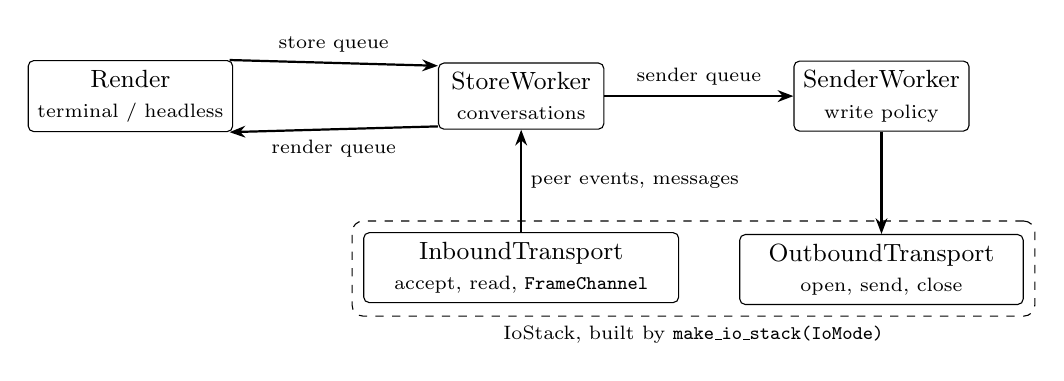
\begin{tikzpicture}[
    box/.style={draw, rounded corners=2pt, minimum height=8mm, minimum width=21mm,
                font=\small, align=center},
    q/.style={-{Stealth[length=2mm]}, thick},
    lbl/.style={font=\scriptsize, midway, fill=white, inner sep=1pt}]
  \node[box] (render) {Render\\\scriptsize terminal / headless};
  \node[box, right=26mm of render] (store) {StoreWorker\\\scriptsize conversations};
  \node[box, right=24mm of store] (sender) {SenderWorker\\\scriptsize write policy};
  \node[box, below=13mm of store, minimum width=40mm] (in) {InboundTransport\\\scriptsize accept, read, \code{FrameChannel}};
  \node[box, below=13mm of sender, minimum width=36mm] (out) {OutboundTransport\\\scriptsize open, send, close};
  \node[draw, dashed, rounded corners, inner sep=4pt, fit=(in)(out),
        label={[font=\scriptsize]below:IoStack, built by \code{make\_io\_stack(IoMode)}}] {};
  \draw[q] (render.20) -- node[font=\scriptsize, above, pos=0.5] {store queue} (store.160);
  \draw[q] (store.200) -- node[font=\scriptsize, below, pos=0.5] {render queue} (render.340);
  \draw[q] (store) -- node[font=\scriptsize, above] {sender queue} (sender);
  \draw[q] (in) -- node[lbl, right=2pt] {peer events, messages} (store);
  \draw[q] (sender) -- (out);
\end{tikzpicture}
\caption{The staged pipeline. Everything above the dashed box is identical in all nine modes.}
\label{fig:pipeline}
\end{figure}

\begin{itemize}
  \item \textbf{\code{StoreWorker}} is single-threaded. It owns conversations and
        subscriptions, and in benchmark (echo) mode it bounces every message back
        to its sender.
  \item \textbf{\code{SenderWorker}} owns all write policy. A transport only opens,
        writes and closes. The policy is:
        \begin{itemize}
          \item what the handshake frames contain;
          \item retries: three attempts, 100\,ms apart, with a 500\,ms
                \code{SO\_SNDTIMEO} on blocking sends;
          \item backpressure: a full transmit buffer (1\,MiB per connection) returns
                \code{WouldBlock} and the message is dropped and counted, with no
                retry or sleep;
          \item port 0 means ``never dial'';
          \item while quitting, nothing is dialled or retried.
        \end{itemize}
  \item \textbf{\code{FrameChannel}} holds the protocol state of one TCP byte stream:
        the frame decoder, the identity learned in the handshake, and forwarding to
        the store. It has no socket. Whatever owns the socket feeds it through
        \code{on\_bytes()} and reports the end through \code{on\_closed()}.
\end{itemize}

\subsection{One controller, two front ends}

\code{ChatController} contains the front-end logic: command parsing, the current
conversation, and the meaning of each store event. It does no input or output of its
own. It writes through a small \code{RenderSink} interface, which has two
implementations:
\begin{itemize}
  \item the interactive terminal UI;
  \item a headless worker that reads commands from stdin and writes one JSON object
        per line.
\end{itemize}
Commands and store events reach the headless worker through the same queue, so they
are handled in one total order. A \code{\#<req-id>} prefix on a command comes back as
\code{"re"} on its eventual reply, and \code{/sync} acts as a barrier that proves the
store has processed every earlier command. This is what makes the end-to-end tests
and the benchmark nodes deterministic.

\subsection{Identifiers and why fds are never keys}

Every id is local to the process that created it. Table~\ref{tab:ids} lists them.
The kernel reuses a file descriptor as soon as it is closed. A table keyed by fd can
therefore deliver a late event for a closed socket to whichever connection has just
been given the same number (an ABA error). Nothing above the pools uses fds:
\begin{itemize}
  \item the pools give out ids that only increase;
  \item handles are never reused, so a stale handle can only miss;
  \item in the split modes, shared ownership keeps an fd open until both pollers
        have removed it.
\end{itemize}

\begin{table}[h]
\centering\small
\begin{tabularx}{\linewidth}{@{}lXl@{}}
\toprule
Id & Purpose & Unique within \\
\midrule
peer id & this node's name for a remote peer & node, forever \\
assigned id & the remote node's name for us, re-presented on reconnect & remote node \\
\code{ChannelRef::connection\_id} & which TCP stream currently holds a peer's rx or tx slot & node, one stream \\
conversation id & one chat history & node, forever \\
handle & what the sender passes to \code{send()} and \code{close()} & one transport, never reused \\
pool id & key inside a connection pool, equal to the handle in pool modes & one pool \\
fd & the kernel descriptor, only inside \code{TcpConnection} & process, \emph{reused} \\
\bottomrule
\end{tabularx}
\caption{Identifier domains.}
\label{tab:ids}
\end{table}

\subsection{Simplex and duplex peer links}

A peer link has an \emph{rx slot} (the stream we read the peer from) and a
\emph{tx slot} (the stream we write to it). Both are stored in the \code{PeerTable}
as a \code{ChannelRef\{connection\_id, handle\}}. The wire format is the same in both
shapes; only the path of the reply differs (Figure~\ref{fig:handshake}):
\begin{itemize}
  \item In \textbf{simplex}, the acceptor dials back to the endpoint the dialler
        advertised, and sends the \code{ConnectAck} on that second connection.
  \item In \textbf{duplex}, the acceptor answers on the connection it accepted.
\end{itemize}
A simplex handshake therefore costs a TCP connect, the \code{Connect}, a second
connect and the \code{Ack}: about 3\,RTT before both sides are ready. A duplex
handshake costs about 2\,RTT.

\begin{figure}[h]
\centering
\begin{minipage}[t]{0.5\linewidth}\vspace{0pt}\centering
  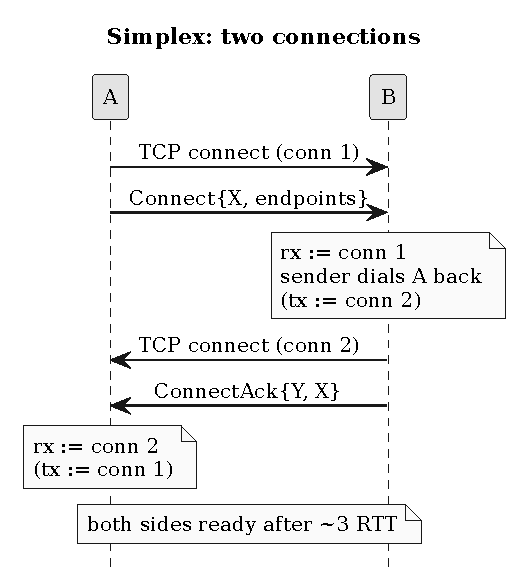
\includegraphics[scale=0.85]{handshake_simplex}
\end{minipage}%
\begin{minipage}[t]{0.5\linewidth}\vspace{0pt}\centering
  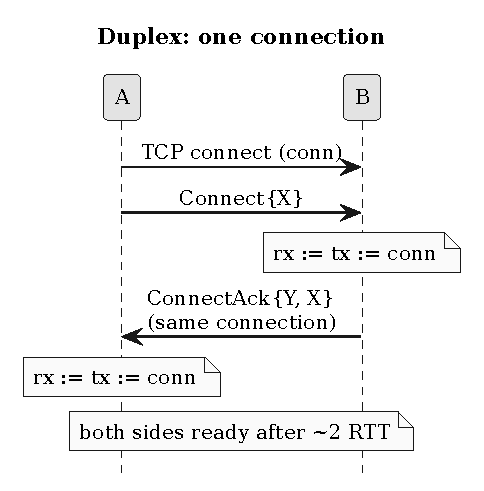
\includegraphics[scale=0.85]{handshake_duplex}
\end{minipage}
\caption{Handshake when A dials B, in the two link shapes. In simplex, A writes on
         conn~1 and B writes on conn~2.}
\label{fig:handshake}
\end{figure}

Three rules hold in both shapes:
\begin{itemize}
  \item \textbf{The newest channel wins a slot.} A release only counts if its
        \code{connection\_id} is still current, so a superseded channel closes
        silently.
  \item \textbf{Exactly one \code{EventPeerDisconnected} per peer.}
  \item \textbf{A channel that closes during its own handshake binds nothing.} A
        small lock and a \code{closing\_} flag guard both the bind and
        \code{on\_closed()}, so a \code{Connect} or \code{Ack} that arrives late on a
        closing channel attaches no slot.
\end{itemize}
The two shapes cannot interoperate: each side would wait for the reply on the wrong
socket. Every node in a run, and the load generator, must use the same shape.

\subsection{Problems met during implementation}
\label{sec:lessons}

Several problems only showed up once the nodes ran under load. Each one taught
something about the socket API or about sharing sockets between threads:
\begin{itemize}
  \item \textbf{File descriptors are reused at once.} With several threads touching
        the same sockets, any table keyed by fd can route a late event to a new
        connection that has been given the old number. The design therefore keeps fds
        inside \code{TcpConnection} and uses ids that only increase everywhere else
        (Table~\ref{tab:ids}).
  \item \textbf{Check-then-act across threads is a race.} The sender first checked
        whether a peer's tx slot was empty and then, in a separate step, decided
        whether to dial. The I/O thread could release the slot in between, and the
        sender then dialled a churned duplex peer at port~0. Such a \code{connect()}
        does not fail at once: it blocks for about 130\,s while the kernel retries the
        SYN. The node stalled in about 1 in 20 duplex runs at 50 reconnects/s. The
        decision has to be made on the same lookup that found the slot empty.
  \item \textbf{A blocking \code{connect()} on a shared thread is expensive.} The
        same blocking dial that caused the stall above is what makes the simplex
        dial-back saturate the sender over a WAN (Section~\ref{sec:res-wan}).
  \item \textbf{Shutdown is a state of the write policy.} After \code{/quit}, a
        backlog of echoes for peers that had already left kept the sender re-dialling
        them, at about 0.2\,s per message. Quitting has to stop all dialling and
        retries, not only the threads.
  \item \textbf{A connection can close during its own handshake.} A \code{Connect}
        or \code{Ack} that arrived late on a closing channel could bind a slot that
        nobody would release. The bind and \code{on\_closed()} now share a small lock
        and a \code{closing\_} flag.
  \item \textbf{Tests need real readiness, not sleeps.} Test binaries running in
        parallel collided on fixed ports, and random ports could be held by another
        process. The tests now redraw a port on a collision and wait for the
        listener's ready callback instead of sleeping.
\end{itemize}

\section{C++ wrappers around the socket API}
\label{sec:wrappers}

Every backend in Section~\ref{sec:backends} is built from a small set of C++ classes
in \code{TcpSocket/}:
\begin{itemize}
  \item \code{TcpListener} and \code{TcpConnection}, which wrap one descriptor each;
  \item \code{PollSet} and \code{TcpConnectionPool}, built on \code{poll(2)};
  \item \code{EpollConnectionPool}, built on \code{epoll(7)};
  \item \code{TxPoller}, a write-only poller with a \code{poll} and an \code{epoll}
        back end.
\end{itemize}
This section describes how these classes call the C functions underneath, and which
rules of the C API shaped them. Table~\ref{tab:syscalls} lists every call and where
it is used.

\begin{table}[h]
\centering\small
\begin{tabularx}{\linewidth}{@{}>{\raggedright\arraybackslash}p{4.4cm}>{\raggedright\arraybackslash}X@{}}
\toprule
C function & Used in \\
\midrule
\code{socket}, \code{bind}, \code{listen}, \code{accept} & \code{TcpListener}; \code{SO\_REUSEADDR} set before \code{bind} \\
\code{socket}, \code{inet\_pton}, \code{connect} & \code{TcpConnection::connect}, always blocking \\
\code{setsockopt}, \code{fcntl} & \code{TcpConnection::apply\_options}: \code{SO\_SNDTIMEO}, \code{SO\_RCVTIMEO}, \code{TCP\_NODELAY}, \code{SO\_KEEPALIVE}, \code{O\_NONBLOCK} \\
\code{send}, \code{recv} & \code{TcpConnection::send}/\code{receive} (blocking, with retries) and \code{send\_once}/\code{receive\_once} (one call, caller's flags) \\
\code{shutdown}, \code{close} & \code{TcpConnection::shutdown} wakes other threads; only the destructor closes \\
\code{poll} & \code{PollSet::wait}, for \code{TcpConnectionPool} and the \code{poll} \code{TxPoller} \\
\code{epoll\_create1}, \code{epoll\_ctl}, \code{epoll\_wait} & \code{EpollConnectionPool} and the \code{epoll} \code{TxPoller} \\
\code{eventfd}, \code{read}, \code{write} & the wake-up descriptor of every poller \\
\bottomrule
\end{tabularx}
\caption{C functions and the wrappers that use them.}
\label{tab:syscalls}
\end{table}

\subsection{Owning a descriptor}

A descriptor is an \code{int} that must be closed exactly once, by exactly one
owner. \code{TcpConnection} and \code{TcpListener} make that an ownership rule of
the type:
\begin{itemize}
  \item the constructor takes the descriptor, and the destructor calls
        \code{close()} if it still holds one;
  \item the classes cannot be copied. A move takes the number with
        \code{std::exchange(other.fd\_, -1)}, so the moved-from object holds $-1$
        and its destructor does nothing;
  \item a connection shared between threads is held in a
        \code{std::shared\_ptr<TcpConnection>}. The last owner to let go closes the
        descriptor, so the number cannot be reused while another thread still uses
        it.
\end{itemize}

The C functions report errors by returning $-1$ and setting \code{errno}. The
wrappers translate \code{errno} at once into a small \code{SocketError} enumeration
(\code{EAGAIN} and \code{EWOULDBLOCK} become \code{WouldBlock}, \code{EINTR}
becomes \code{Interrupted}, and so on). They return it in a
\code{std::expected}, so the caller has to look at the error before it can use the
value. Only the \code{TcpListener} constructor throws, because a listener that
could not bind is not a usable object.

Addresses are built as a value-initialised \code{sockaddr\_in\{\}}, which also
zeroes the \code{sin\_zero} padding, and filled with \code{htons} and
\code{inet\_pton}. A failed \code{inet\_pton} is reported as a bad address before
any system call is made.

\subsection{Socket options}

\code{TcpConnection} stores its options and applies them in one place,
\code{apply\_options()}:
\begin{itemize}
  \item \code{SO\_SNDTIMEO} and \code{SO\_RCVTIMEO} take a \code{struct timeval}. A
        zero value means ``no timeout'', so the same code both sets and clears them.
  \item \code{TCP\_NODELAY} turns off Nagle's algorithm. Without it, a small frame
        could wait for the acknowledgement of the previous one. Every connection in
        the node sets it.
  \item \code{SO\_KEEPALIVE} lets the kernel notice a peer that has vanished without
        closing.
  \item \code{O\_NONBLOCK} is a flag on the open file, not a socket option. It is
        read with \code{fcntl(F\_GETFL)} and written back with \code{F\_SETFL}, so the
        other flags are kept.
\end{itemize}
The \code{with\_*()} setters only record the values, and the next \code{send} or
\code{receive} applies them. This is convenient for one thread. It is a data race
when a reader and a writer share the socket, because both would check and set the
``applied'' flag. Connections handed to a pool or a \code{TxPoller} are therefore
configured with \code{apply\_options\_now()} first; after that, the I/O calls only
read the flag.

\subsection{Reading and writing}

There are two pairs of I/O calls:
\begin{itemize}
  \item \code{send()} and \code{receive()} serve the blocking modes. They loop over
        \code{::send} and \code{::recv}, retry on \code{EINTR} and \code{EAGAIN} if
        retries were configured, and turn a \code{recv} that returns 0 into
        \code{ConnectionClosed}.
  \item \code{send\_once()} and \code{receive\_once()} are for the pollers. They make
        exactly one call with the flags the caller passes (\code{MSG\_DONTWAIT}),
        report \code{WouldBlock} as it is, and return a 0-byte read as 0, so the pool
        can treat it as end of stream.
\end{itemize}
Every \code{send} adds \code{MSG\_NOSIGNAL}. Without it, writing to a connection the
peer has closed raises \code{SIGPIPE}, which kills the whole process. With it, the
call simply fails with \code{EPIPE}.

A \code{send} may write only part of the buffer. The blocking outbound path wraps it
in \code{send\_all()}, which continues from where the previous call stopped. On a
blocking socket with \code{SO\_SNDTIMEO}, a send that waits too long fails with
\code{EAGAIN}, which the sender treats like a full buffer.

In \mode{threads} and \mode{pool-sender}, each reader thread blocks in
\code{receive()} with a 200\,ms \code{SO\_RCVTIMEO}. When the timeout expires,
\code{recv} fails with \code{EAGAIN}. The reader treats that as ``nothing yet'',
updates its heartbeat for the watchdog, and calls \code{recv} again.

\subsection{Ending a connection: \texttt{shutdown} before \texttt{close}}

Closing a descriptor that another thread is blocked on does not reliably wake that
thread. Worse, the number becomes free at once and can be given to a new connection
while the old thread still holds it. The wrappers therefore separate the two steps:
\begin{itemize}
  \item \code{TcpConnection::shutdown()} calls \code{shutdown(fd, SHUT\_RDWR)}. A
        thread blocked in \code{recv} on that socket then returns 0, as if the peer
        had closed. The descriptor stays valid, so no other connection can get its
        number. \code{ENOTCONN} is not treated as an error, because it only means
        the peer was already gone.
  \item \code{close()} is called only by the destructor, once no thread can use the
        socket any more.
\end{itemize}
The watchdog uses this to evict a blocking reader. The split modes use it so that a
failed write on the write thread shows up on the read thread as end of stream. The
pools call it whenever they drop a connection.

\code{accept()} on a listening socket cannot be woken this way. To stop a listener
blocked in \code{accept}, the node sets a stop flag and then connects to its own
listening port. \code{accept} returns, the loop sees the flag, and it closes the
wake-up connection.

\code{connect()} is always blocking (Section~\ref{sec:lessons}). The wrapper refuses
port~0 before calling it, because Linux does not reject a connection to port~0: the
SYN simply goes unanswered and the call blocks for about 130\,s of retries.

\subsection{The \texttt{poll} wrapper}
\label{sec:wrap-poll}

\code{poll()} reads an array of \code{struct pollfd} while it blocks, so no other
thread may change that array during the call. \code{PollSet} solves this with two
copies of the state:
\begin{itemize}
  \item a \emph{desired} table, \code{id}~$\to$~\code{pollfd}, which any thread may
        change under the pool's mutex (\code{upsert()} and \code{erase()});
  \item the \emph{kernel} array \code{fds\_}, which only the I/O thread touches. It
        is rebuilt from the desired table (\code{prepare()}), under the mutex, and
        only when that table has changed.
\end{itemize}
The I/O thread then releases the mutex and calls \code{::poll(fds\_, n, timeout)}.
The timeout is the time until the next sweep for idle connections. A call that fails
with \code{EINTR} is repeated.

Slot~0 of the array always holds an \code{eventfd} created with
\code{EFD\_NONBLOCK | EFD\_CLOEXEC}. When another thread adds a connection, queues a
write or closes the pool, it writes the 8-byte value 1 to that descriptor. The
blocked \code{poll} returns, and the I/O thread reads the counter back to zero and
rebuilds the array if needed.

On return, \code{for\_each\_ready()} walks the \code{revents} of every entry,
starting after the socket it served last, so a busy socket cannot starve the others:
\begin{itemize}
  \item \code{POLLOUT} with queued bytes: flush them with \code{send\_once};
  \item \code{POLLIN}: one \code{receive\_once} into the caller's buffer;
  \item \code{POLLERR}, \code{POLLHUP} or \code{POLLNVAL}: drop the connection and
        report it as closed.
\end{itemize}
\code{POLLOUT} is in the desired table only while a connection has queued bytes.
Otherwise every connection with free buffer space would be reported as writable on
every call.

\code{receive()} returns as soon as it has one chunk from one socket. The next call
makes a new \code{poll()}. With many sockets, every message read therefore costs one
scan of the whole array in the kernel and one walk over the \code{revents} in the
pool. This is the cost that grows with idle peers in S2.

\subsection{The \texttt{epoll} wrapper}

\code{EpollConnectionPool} uses the three \code{epoll} calls:
\begin{itemize}
  \item \code{epoll\_create1(EPOLL\_CLOEXEC)} creates the instance once, in the
        constructor. Its \code{eventfd} is registered first, with the token 0 in
        \code{epoll\_event.data.u64}.
  \item \code{epoll\_ctl} keeps the kernel's interest list up to date:
        \code{EPOLL\_CTL\_ADD} with \code{EPOLLIN} when a connection arrives,
        \code{EPOLL\_CTL\_MOD} to add or remove \code{EPOLLOUT} (only when the
        interest actually changes, which saves a system call), and
        \code{EPOLL\_CTL\_DEL} when it leaves. These calls are safe while the I/O
        thread is blocked in \code{epoll\_wait}, so no second copy of the state is
        needed.
  \item \code{epoll\_wait} fills a preallocated array of \code{max\_connections + 2}
        events.
\end{itemize}

Two details of the C API matter here:
\begin{itemize}
  \item \textbf{The event carries the connection id, not the fd.} Ids start at 1 and
        are never reused, so the token 0 can mean the \code{eventfd}, and an event
        for a connection removed in the meantime cannot reach a new connection with
        the same descriptor number.
  \item \textbf{\code{EPOLL\_CTL\_DEL} comes before \code{shutdown} and the release.}
        The kernel removes a descriptor from an epoll set by itself only when every
        reference to the underlying open file is closed. A connection shared with a
        \code{TxPoller} may outlive the pool's reference, so the pool removes it
        explicitly.
\end{itemize}

The pool is level-triggered: it does not set \code{EPOLLET}. A socket that still has
unread data is reported again by the next \code{epoll\_wait}, so the pool may read
one chunk and return. With edge triggering it would have to read until
\code{EAGAIN}, or it could miss data. Like the \code{poll} pool, \code{receive()}
serves one ready socket per call. Its fairness cursor indexes the events array of
the \emph{previous} call, whose contents are different each time, so it is not the
strict round robin of \code{PollSet}. This may contribute to \code{epoll}'s worse
tail at 1,024 busy peers (Section~\ref{sec:res-fanin}); we have not tested it.

\subsection{Writes through a pool, and the \texttt{TxPoller}}

All three pollers (\code{TcpConnectionPool}, \code{EpollConnectionPool} and
\code{TxPoller}) write in the same way:
\begin{enumerate}
  \item If nothing is queued for the connection, \code{send\_once(MSG\_DONTWAIT)}
        writes as much as the kernel accepts at once.
  \item Whatever the kernel did not accept is appended to the connection's
        \code{tx\_buffer}, and writability is armed: \code{POLLOUT} in the desired
        table, or \code{EPOLLOUT} through \code{epoll\_ctl}.
  \item When the socket becomes writable, the buffer is flushed until it is empty
        or the kernel says \code{EAGAIN} again. Once it is empty, writability is
        disarmed.
  \item A message that would push the buffer past 1\,MiB is refused with
        \code{WouldBlock}, and nothing of it is queued. This is the backpressure drop
        of Section~\ref{sec:arch}.
\end{enumerate}
The buffer keeps an offset of its first unsent byte, and it is compacted only once
that offset passes half the buffer, so appending stays cheap.

The \code{TxPoller} of the split modes runs the same algorithm on its own thread. It
never reads, and it watches a socket only while that socket has queued bytes, so its
set is usually empty. Unlike the read pools, it handles every ready descriptor
returned by one \code{poll} or \code{epoll\_wait} (up to 64 for \code{epoll}) before
it waits again.

\section{The nine I/O backends}
\label{sec:backends}

Table~\ref{tab:modes} summarises the nine backends. Seven base threads are present in
every mode: main/render, the stdin reader, the logger, the store, the sender, the
listener and metrics.

\begin{table}[h]
\centering\small
\begin{tabularx}{\linewidth}{@{}lcc>{\raggedright\arraybackslash}Xlc@{}}
\toprule
\code{-{}-io=} & conn./peer & fds/peer & read path & write path & threads \\
\midrule
\mode{threads}      & 2 & 2 & blocking reader thread per connection & blocking, on the sender & $8+N$ \\
\mode{pool-sender}  & 2 & 2 & as \mode{threads} & non-blocking pool + pump & $9+N$ \\
\mode{(e)poll} & 2 & 2 & one pool, one I/O thread & same pool & 8 \\
\mode{(e)poll-duplex} & 1 & 1 & one pool, one I/O thread & same pool, same socket & 8 \\
\mode{(e)poll-split} & 1 & 1 & rx pool + I/O thread & \code{TxPoller} + tx thread & 9 \\
\mode{peer-threads} & 1 & 2 & one owner thread per peer & one-connection pool & $8+N$ \\
\bottomrule
\end{tabularx}
\caption{Backends. \mode{(e)poll} stands for both the \code{poll} and \code{epoll} variant. $N$ is the number of peers. ``fds/peer'' excludes the node's fixed descriptors.}
\label{tab:modes}
\end{table}

\subsection{\mode{threads} and \mode{pool-sender}}

\code{ListenerWorker} accepts connections in a blocking loop and starts one
\code{ReaderWorker} thread per connection. Each reader waits in \code{receive()} with a
200\,ms timeout and bumps a heartbeat counter.

\code{WatchdogWorker} looks after the readers:
\begin{itemize}
  \item It scans every 100\,ms and joins readers that have finished.
  \item A reader whose heartbeat has not moved for 10 scans (1\,s) is treated as
        wedged; the watchdog shuts its socket down to unblock it.
  \item It enforces \code{-{}-max-peers}. Once the cap is exceeded, the least recently
        active readers are evicted first.
\end{itemize}

The two modes differ only in how they write:
\begin{itemize}
  \item \mode{threads} writes with blocking \code{send}s on the sender thread. A peer
        that stops reading stalls that thread for up to 500\,ms per attempt.
  \item \mode{pool-sender} still dials with a blocking \code{connect}, but then hands
        the socket to a \code{TcpConnectionPool}. Every send is non-blocking, and
        whatever doesn't fit is queued, up to 1\,MiB. A pump thread drives the pool,
        flushing queued bytes and noticing dead sockets.
\end{itemize}

\subsection{\mode{poll} and \mode{epoll}, simplex and duplex}

All four modes are \code{MultiplexedIo<Pool>}: one pool holds every connection, and
one I/O thread loops on \code{pool.receive()}. A single call returns bytes from any
readable connection and flushes queued writes on any writable one. \code{POLLOUT}
(or \code{EPOLLOUT}) is armed only while a transmit buffer holds data.

\code{registry\_} maps pool ids to \code{FrameChannel}s. Whoever adds a connection
holds \code{registry\_mutex\_} across both the pool insert and the registry insert, so
the I/O thread can never receive bytes for an id it cannot find.

The two pools differ in how they track sockets:
\begin{itemize}
  \item \code{TcpConnectionPool} keeps a desired-state table and rebuilds its
        \code{pollfd} array before a \code{poll()} whenever that table has
        changed. Other threads wake it through
        an \code{eventfd(2)}. A round-robin cursor decides which ready socket is
        served first.
  \item \code{EpollConnectionPool} calls \code{epoll\_ctl} directly, even while
        another thread is blocked in \code{epoll\_wait}. Its wake-up eventfd uses the
        reserved token 0 (\code{kWakeToken}), and it keeps a fairness cursor over the
        ready events.
\end{itemize}

The \emph{Dual} model (\mode{poll}, \mode{epoll}) keeps two connections per peer in
one pool, with capacity $2\times$\code{max\_peers}. Accepted sockets have a channel;
dialled ones carry writes only. The \emph{Duplex} model gives every connection a
channel, whether it was accepted or dialled, and the \code{ConnectAck} goes back on
the same handle. Its capacity is \code{max\_peers}${}+16$. Duplex halves the sockets
and avoids the dial-back.

\subsection{\mode{poll-split} and \mode{epoll-split}}

These modes use the same duplex link logic, but read and write each socket on
different threads:
\begin{itemize}
  \item Each connection is a \code{shared\_ptr<TcpConnection>} held by three owners:
        the rx pool (which only reads it), a \code{TxPoller} (which only writes it)
        and the registry.
  \item The \code{TxPoller} has its own thread and waits for writability only on
        connections that have queued bytes.
  \item Socket options are applied eagerly (\code{apply\_options\_now()}) before the
        connection is shared, so neither thread changes them later.
  \item A fatal write calls \code{shutdown(SHUT\_RDWR)}. The rx pool then sees EOF and
        reports the disconnect, so disconnects are always reported from the read
        side.
\end{itemize}

\subsection{\mode{peer-threads}}

Each peer is a \emph{link}: a one-connection \code{TcpConnectionPool} driven by its
own owner thread (\code{pt-<handle>}).
\begin{itemize}
  \item \textbf{Reads and flushing:} the owner thread reads the socket and flushes
        queued writes.
  \item \textbf{Immediate writes:} the shared sender writes through
        \code{pool.send()} under the pool's mutex, so frames never interleave.
  \item \textbf{Ending a link:} the owner thread is the only caller of
        \code{on\_closed()}, so the link is reported gone exactly once. That holds
        whichever of the four triggers comes first: the peer closing, a malformed
        frame, the sender's \code{close()}, or a watchdog eviction.
  \item \textbf{Cap:} links count against \code{-{}-max-peers} through the shared
        watchdog, which evicts the link with the oldest \code{last\_read\_ns}. Stall
        detection is turned off, because an idle owner legitimately blocks in
        \code{receive()}.
  \item \textbf{No restarts:} an evicted owner thread is joined and gone. The peer
        can only come back as a new link, with a new handle and \code{connection\_id}.
\end{itemize}

\textbf{Limitations.} Retries are a 100\,ms sleep on the shared sender thread, and
\code{open()} performs a blocking \code{connect()} on that same thread.
Section~\ref{sec:res-churn} measures the cost of the first.

\section{Instrumentation and benchmark methodology}
\label{sec:method}

\subsection{Inside the node}

The node keeps lock-free counters (relaxed atomics), including:
\begin{itemize}
  \item frames in and out, and accepts;
  \item send failures and backpressure drops;
  \item reconnects and evictions;
  \item queued sends and flushes;
  \item high-water marks of the render, store and sender queues.
\end{itemize}
With \code{-{}-metrics}, a metrics thread writes one JSONL snapshot per second. Each
snapshot adds \code{getrusage(2)} figures (user and system CPU time, voluntary and
involuntary context switches, maximum RSS) and thread and fd counts from
\code{/proc/self}. Every node thread is named, so a hang dump identifies each thread.

\paragraph{CPU usage.} \code{getrusage(RUSAGE\_SELF)} returns the user time
$u$ and system time $s$ consumed so far by \emph{all} threads of the process. Given
two snapshots taken at wall-clock times $t_a$ and $t_b$, the node's CPU usage over
that interval is
\begin{equation}
\mathrm{CPU} = 100\% \times \frac{(u_b + s_b) - (u_a + s_a)}{t_b - t_a}.
\label{eq:cpu}
\end{equation}
The numerator is CPU time and the denominator is elapsed time, so the ratio is the
average number of cores the process kept busy: 100\% is one core fully used. The node
is pinned to two CPUs, so its ceiling is 200\%. This is the usual way to compute a
process's CPU usage on Linux, whether the times come from \code{getrusage} or from the
\code{utime} and \code{stime} fields of \code{/proc/<pid>/stat}~\cite{poll,so-cpu}.
$t_a$ and $t_b$ are the snapshots that bound the measurement window.

\paragraph{Context switches.} The same \code{getrusage(RUSAGE\_SELF)} call returns
two counters, summed by the kernel over all threads of the process:
\begin{itemize}
  \item \code{ru\_nvcsw}, \emph{voluntary} context switches: a thread gave up the CPU
        itself because it had to wait, for example blocking in \code{recv},
        \code{poll}, \code{epoll\_wait}, on a mutex or on a queue's condition
        variable;
  \item \code{ru\_nivcsw}, \emph{involuntary} context switches: the scheduler took
        the CPU away from a thread that was still runnable, because its time slice
        ran out or another thread had to run.
\end{itemize}
Both counters only grow, so they are turned into rates in the same way as
Equation~\ref{eq:cpu}:
\begin{equation}
\text{voluntary rate} = \frac{\mathit{nvcsw}_b - \mathit{nvcsw}_a}{t_b - t_a},
\qquad
\text{involuntary rate} = \frac{\mathit{nivcsw}_b - \mathit{nivcsw}_a}{t_b - t_a}.
\end{equation}
A high voluntary rate means threads often sleep and wake, for example once per
message. At 1,024 peers the thread modes switch voluntarily 89--107 thousand times
per second, against 6--16 thousand for the modes with one I/O thread. A high
involuntary rate means there were more runnable threads than CPUs.

\subsection{The load generator}
\label{sec:gen}

\code{stressgen} is a single-threaded \code{epoll} client. It simulates many peers that
speak the same protocol as the node, in either link shape (\code{-{}-duplex}).
\begin{itemize}
  \item \textbf{RTT:} each message embeds its send time, and RTT is measured when the
        node's echo arrives, on the same clock. Times are recorded in a log-bucketed
        histogram with 32 sub-buckets per power of two, so a quantile is
        over-estimated by less than 3.125\%.
  \item \textbf{What counts:} only messages sent inside the measurement window, with
        a short grace period for late echoes.
  \item \textbf{Load:} open loop (a fixed \code{-{}-rate} per peer) or closed loop (a
        \code{-{}-window} of outstanding messages per peer).
  \item \textbf{Peer types:} besides active peers, it can run idle peers and slow
        peers (receive buffer 4\,KiB, never read).
  \item \textbf{Churn:} at a fixed rate (\code{-{}-churn}, reconnects per second), the
        generator closes a randomly chosen \emph{ready} peer and redials it at once.
        The schedule is open loop: it does not wait for earlier redials to finish. If
        no peer is ready when a churn event is due, the event is skipped.
  \item \textbf{Handshakes:} it records handshake latency from TCP connect to Ready.
\end{itemize}

\subsection{The harness}

\code{run\_matrix.py} runs the experiment as a matrix of \emph{cells}. A cell is one
scenario, one swept value, one mode and one repetition. For each cell it:
\begin{enumerate}
  \item starts the node in headless echo mode with the chosen \code{-{}-io} mode and
        \code{-{}-metrics}, pinned with \code{taskset} to CPUs 0--1, and waits for the
        node's \code{ready} event on its JSON output;
  \item starts \code{stressgen}, pinned to CPUs 4--7, which dials every simulated peer
        (in batches, so the accept backlog does not overflow) and waits until all of
        them have completed the handshake or a ramp deadline has passed;
  \item lets the generator run a 5\,s warm-up and then a 20\,s measurement window,
        after which it writes its result file;
  \item sends \code{/quit} to the node on its standard input and waits up to 30\,s for
        the reply \code{bye} and for the process to exit. A node that does not exit
        has the state of every thread recorded from \code{/proc} and is then killed;
  \item writes a metadata file with the cell's parameters, the build stamp (commit,
        uncommitted changes, binary hash, build type), the node's exit status and the
        result of the validity checks below.
\end{enumerate}
The CPUs 0--1 and 4--7 are separate physical cores of an Intel Core Ultra~7 155H,
under WSL2 (Linux 6.6). The order of the modes is shuffled for every (scenario, value,
repetition), so slow drift on the machine is spread across modes rather than biasing
one. The script refuses non-Release builds, and when an interrupted run is resumed it
refuses to mix cells from different builds.

Table~\ref{tab:scenarios} lists the scenarios.

\begin{table}[h]
\centering\small
\begin{tabularx}{\linewidth}{@{}llXl@{}}
\toprule
Scenario & Swept & Other load & Network \\
\midrule
S1 fan-in & active peers 1, 8, 64, 256, 1024 & 100 msg/s per peer, 64\,B & loopback \\
S2 idle-heavy & idle peers 0, 100, 300, 1000 & 8 active $\times$ 500 msg/s & loopback \\
S3 slow consumers & slow peers 0, 1, 4 & 16 active $\times$ 200 msg/s & loopback \\
S4 churn & reconnects/s 0, 10, 50 & 64 peers $\times$ 50 msg/s & loopback \\
S5 throughput & size 32\,B, 4\,KiB, 64\,KiB & 8 peers, closed loop, window 16 & loopback \\
S6a WAN churn & RTT 0, 4, 20, 30, 40, 50\,ms & 32 $\times$ 100 msg/s, 256\,B, 16 reconnects/s & veth + netem \\
S6c WAN churn, half & RTT 50\,ms & as S6a, 8 reconnects/s & veth + netem \\
S6b WAN bottleneck & 1000, 200, 50\,Mbit/s & 32 peers, closed loop, window 8, 16\,KiB & veth, 4\,ms RTT \\
S7 capped fan-in & \code{-{}-max-peers} 64, 128, 256, 1040 & 1024 peers $\times$ 100 msg/s & loopback \\
\bottomrule
\end{tabularx}
\caption{Scenarios: 32 swept values $\times$ 9 variants $\times$ 3 repetitions = 864 cells.}
\label{tab:scenarios}
\end{table}

\paragraph{WAN lab.} The S6 cells run inside an unprivileged \code{unshare}
namespace. The node and the generator are joined by a veth pair with MTU 1500 and
offloads disabled. netem~\cite{netem} delay is split evenly between the two
directions, so the configured RTT is their sum. The S6b rate limit applies only to
the node's egress.

\subsection{Analysis and validity}

\code{analyze.py} aligns the node's metrics window with the generator's monotonic
window bounds. From that window it computes CPU usage (Equation~\ref{eq:cpu}) and
context-switch rates per cell, and it reports the median and inter-quartile range over the valid
repetitions.

A cell counts as \emph{degraded}, and is left out of the medians, if any of these
checks fails:
\begin{itemize}
  \item not every peer became ready (at least 90\% with churn; the cap rule in S7);
  \item an open-loop cell offered less than 98\% of its nominal load;
  \item there were connect failures (outside S7), bad frames or skipped sends;
  \item the node stalled: its \code{frames\_in} stopped growing within 3\,s of the
        window's end.
\end{itemize}
Overload is a result, not a failure. A cell that delivered a fraction of its load with
huge latency is reported as the point where that mode breaks.

\subsection{The measured run}

All results come from one run of the full matrix: 864 cells from one clean Release
build (\code{-O3}). Every cell completed, and every node exited with status 0 and no
hang. 840 cells pass every validity check. The 24 degraded cells are all simplex S6a
cells at RTT 40 and 50\,ms (Section~\ref{sec:res-wan}). The build and the location of
the raw data are listed in Appendix~\ref{app:repro}.

\subsection{Limitations}

\begin{itemize}
  \item The node and the generator share one WSL2 host, and loopback RTT includes the
        generator's own processing time.
  \item CPU and context switches are measured for the node only, without its softirq
        share. Threads and fds are sampled once a second.
  \item The node has two CPUs. That is where the thread-per-connection ceiling falls;
        with more cores it would move up.
  \item There is no counter for outbound bytes.
  \item Handshake statistics only include peers that completed a handshake, so they
        carry survivorship bias.
  \item The generator's slow peers never made the duplex shapes queue writes
        (Section~\ref{sec:res-slow}).
\end{itemize}

\section{Results}
\label{sec:results}

All values are medians over three repetitions; the shaded bands in the figures are
the inter-quartile range. Figures share one encoding: colour gives the concurrency
family (blue for threaded, orange for \code{poll}, green for \code{epoll}), and line
style and marker give the socket topology (solid for simplex, dashed for duplex,
dotted for split). Values are comparable only within one scenario and one swept value.

%-----------------------------------------------------------------------------
\subsection{S1: fan-in}
\label{sec:res-fanin}

\begin{figure}[h]
\centering
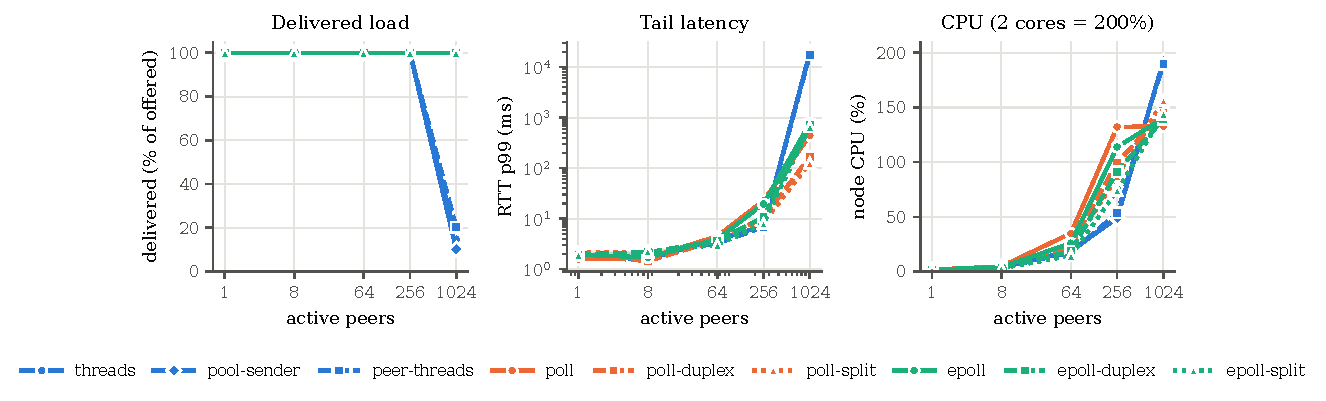
\includegraphics[width=\linewidth]{s1_fanin}
\caption{S1. Each peer offers 100 msg/s. The node has two CPUs (200\%).}
\label{fig:s1}
\end{figure}

\finding{Thread-per-connection collapses at 1,024 peers.} Table~\ref{tab:s1-1024}
shows the result. \mode{threads}, \mode{pool-sender} and \mode{peer-threads} deliver
10.4--20.8k of the 102.4k msg/s offered. Their median RTT is 16--19\,s, they run about
1,030 threads, and they use both cores. Every multiplexed mode delivers the whole load
with no loss. Each runnable reader thread competes for two CPUs, and the scheduler
cannot keep up.

\begin{table}[h]
\centering\small
\begin{tabular}{@{}lrrrrrrr@{}}
\tablebody{tables/s1_1024.tex}
\end{tabular}
\caption{S1 at 1,024 active peers (102.4k msg/s offered).}
\label{tab:s1-1024}
\end{table}

\finding{Duplex halves the descriptors.} At 1,024 peers the duplex and split modes
use about 1,031 fds, against 2,055 for \mode{poll}/\mode{epoll}. \mode{peer-threads}
also uses two per peer, because each link's pool has an eventfd.

\finding{Below the ceiling, threads are the cheapest mode.} At 256 peers
(Table~\ref{tab:s1-256}), \mode{threads}, \mode{pool-sender} and \mode{peer-threads}
use 49--54\% CPU, with a p99 of 6.8--7.2\,ms. \mode{poll} and \mode{epoll} use
114--132\% for a p99 of about 20\,ms. The duplex and split modes fall in between.
A blocked reader costs almost nothing, and the work of the active ones spreads over both
cores. A single I/O thread makes at least one system call per ready socket, and all
of them run on one core.

\begin{table}[h]
\centering\small
\begin{tabular}{@{}lrrrr@{}}
\tablebody{tables/s1_256.tex}
\end{tabular}
\caption{S1 at 256 active peers (25.6k msg/s offered; every mode delivers it).}
\label{tab:s1-256}
\end{table}

\finding{An unexplained ordering at 1,024 peers.} The poll-based duplex and split
modes have the lowest latency: p50 60--76\,ms and p99 126--168\,ms. Their epoll twins
are at 147--159\,ms p50 and 654--721\,ms p99. The ordering holds in all three
repetitions. The data does not explain it. One plausible mechanism is the order in
which each pool serves ready sockets: \code{poll}'s round-robin cursor against
\code{epoll}'s ready list. We report this as an observation, not a finding.

%-----------------------------------------------------------------------------
\subsection{S2: idle connections}

\begin{figure}[h]
\centering
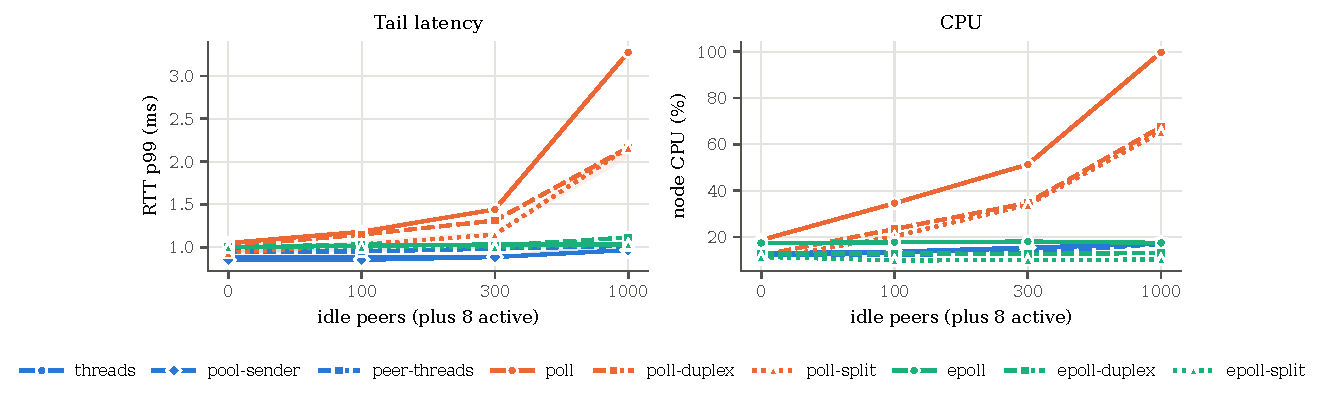
\includegraphics[width=\linewidth]{s2_idle}
\caption{S2. Eight active peers at 500 msg/s each, plus idle peers.}
\label{fig:s2}
\end{figure}

\finding{\code{poll()} pays for idle sockets; \code{epoll} does not.}
Figure~\ref{fig:s2} shows the cost. From 0 to 1,000 idle peers:
\begin{itemize}
  \item \mode{poll}'s p99 rises from 1.05 to 3.28\,ms and its CPU from 19\% to 100\%,
        because every \code{poll()} call scans the whole \code{pollfd} array, and the
        pool makes one call per chunk it reads (Section~\ref{sec:wrap-poll});
  \item the poll duplex and split modes have half as many sockets to scan and pay
        about half (about 65\% CPU);
  \item every \code{epoll} variant stays flat, at about 1.0\,ms p99 and 10--17\% CPU.
\end{itemize}
In the thread modes each idle peer costs a thread (1,016 threads), but latency stays
flat: a blocked thread uses no CPU between its 200\,ms heartbeat wake-ups.

%-----------------------------------------------------------------------------
\subsection{S3: slow consumers}
\label{sec:res-slow}

\begin{figure}[h]
\centering
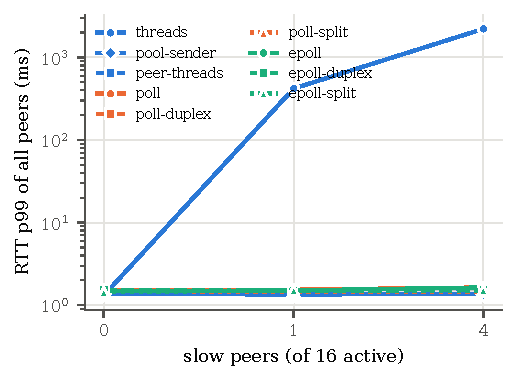
\includegraphics[width=0.55\linewidth]{s3_slow}
\caption{S3. The p99 of all peers when some stop reading.}
\label{fig:s3}
\end{figure}

\finding{Only a blocking sender lets one slow reader stall everyone.} One slow peer
raises \mode{threads}' p99 for \emph{all} peers from 1.3\,ms to 419\,ms, and four slow
peers raise it to 2.2\,s (Figure~\ref{fig:s3}). The sender thread waits up to
500\,ms per blocking write. Every other mode stays at 1.3--1.6\,ms. The pooled simplex
modes queue about 2,045 writes per slow peer but never reach the 1\,MiB cap within
20\,s, so nothing is dropped.

\textbf{Caveat.} The duplex, split and \mode{peer-threads} modes record no queued
writes at all, even with a 4\,KiB receive buffer on the slow peers. For these shapes
the result shows that no peer stalled, not that a slow reader was isolated under
backpressure.

%-----------------------------------------------------------------------------
\subsection{S4: churn}
\label{sec:res-churn}

\begin{figure}[h]
\centering
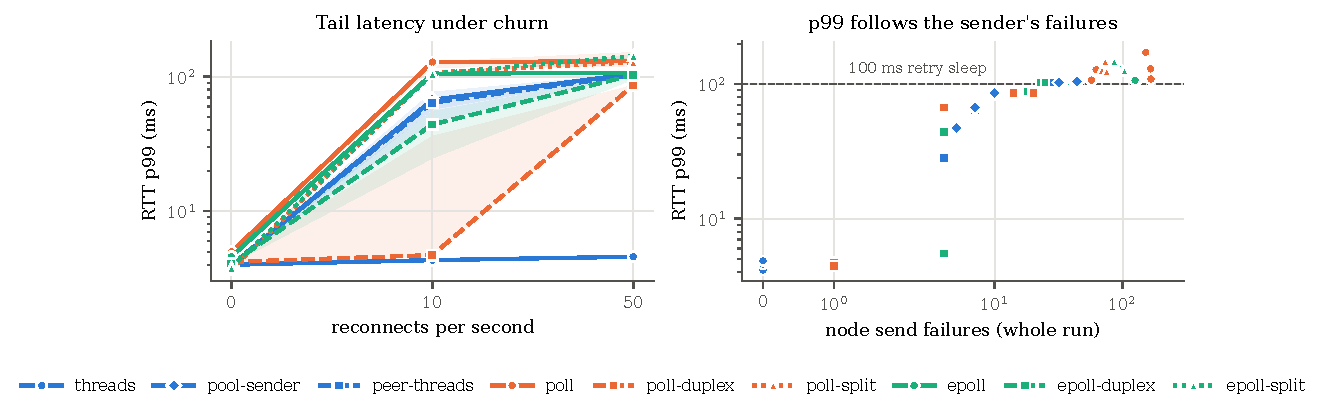
\includegraphics[width=\linewidth]{s4_churn}
\caption{S4. Left: p99 against churn. Right: each valid repetition at churn 10 and 50,
         plotting the node's send failures against p99.}
\label{fig:s4}
\end{figure}

\finding{Churn moves the tail, and the tail follows the sender's failures.} At churn
of 10 reconnects/s and above, most modes reach a p99 of 44--143\,ms. Only
\mode{threads} stays at about 4.5\,ms, and \mode{poll-duplex} does too at churn 10.
Table~\ref{tab:s4} and Figure~\ref{fig:s4} show that p99 follows the number of failed
sends. A failed send (\code{ConnectionNotFound} for a handle that has just been
closed) makes the sender sleep 100\,ms before retrying, on the single thread that
writes for every peer. Every other peer waits with it:
\begin{itemize}
  \item cells with zero or one failure keep a p99 of about 5\,ms;
  \item a handful of failures already raises p99 in some repetitions, and from about
        ten failures per run p99 sits at or above the 100\,ms sleep;
  \item the simplex \mode{poll} and \mode{epoll} modes fail most often (125--166 times
        at churn 50), and they are the only modes whose \emph{median} also rises, to
        32\,ms and 13\,ms.
\end{itemize}

\begin{table}[h]
\centering\small
\begin{tabular}{@{}lllrrr@{}}
\tablebody{tables/s4.tex}
\end{tabular}
\caption{S4: the node's send failures for each of the three repetitions, against tail latency.}
\label{tab:s4}
\end{table}

\finding{Threaded reads do not prevent this.} \mode{pool-sender} and
\mode{peer-threads} read on their own threads, with isolated descriptors, and still
reach a p99 of 64--105\,ms. \mode{threads} has no failures at all. The likely
mechanism, which we have not proven, is that its blocking \code{send()} on a
just-closed socket still succeeds into the kernel buffer. The echo is then lost
silently instead of retried, which also gives \mode{threads} the lowest loss. The pool
modes notice the EOF first, so their next send fails and the sender sleeps. The split
modes fail more often than the duplex modes (69--103 against 14--25 at churn 50). The
same 100\,ms signature appears as the handshake p99 at RTT 0 in S4 and S6a.

%-----------------------------------------------------------------------------
\subsection{S5: throughput ceiling}

\begin{figure}[h]
\centering
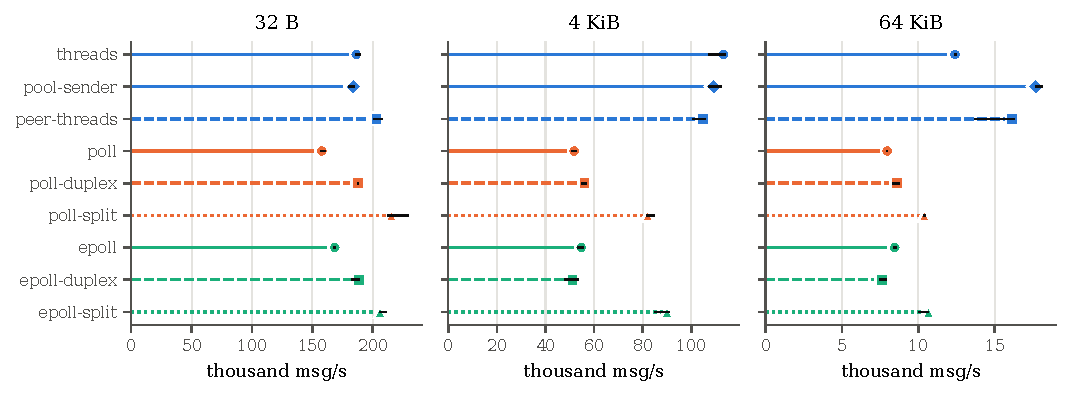
\includegraphics[width=\linewidth]{s5_throughput}
\caption{S5. Closed loop, 8 peers with 16 messages outstanding each. Black whiskers are the IQR.}
\label{fig:s5}
\end{figure}

\begin{table}[h]
\centering\small
\begin{tabular}{@{}lrrrr@{}}
\tablebody{tables/s5.tex}
\end{tabular}
\caption{S5: throughput in thousands of messages per second.}
\label{tab:s5}
\end{table}

\finding{The single I/O thread is the ceiling.} At 4 and 64\,KiB, every mode with one
I/O thread plateaus at about 122--144\% CPU and 51--56k msg/s (4\,KiB), or
7.6--8.6k msg/s (64\,KiB). The thread modes reach 170--180\% and the highest
throughput:
\begin{itemize}
  \item 105--113k msg/s at 4\,KiB;
  \item 17.7k msg/s for \mode{pool-sender} and 16.2k for \mode{peer-threads} at
        64\,KiB.
\end{itemize}

\finding{A separate write thread pays off once that thread is the bottleneck.}
Compared with their duplex twins, the split modes gain:
\begin{itemize}
  \item at 4\,KiB, with only 8 peers: 46\% (\mode{poll}) and 76\% (\mode{epoll});
  \item at 64\,KiB: 21\% and 40\%;
  \item at 32\,B: 15\% and 9\%.
\end{itemize}

\finding{Simplex buys no throughput.} At 32\,B, \mode{poll} and \mode{epoll} are
slower than their duplex versions: 158k against 188k, and 169k against 189k msg/s. At
4 and 64\,KiB the two shapes are within noise.

%-----------------------------------------------------------------------------
\subsection{S6: WAN churn and bottleneck}
\label{sec:res-wan}

\begin{figure}[h]
\centering
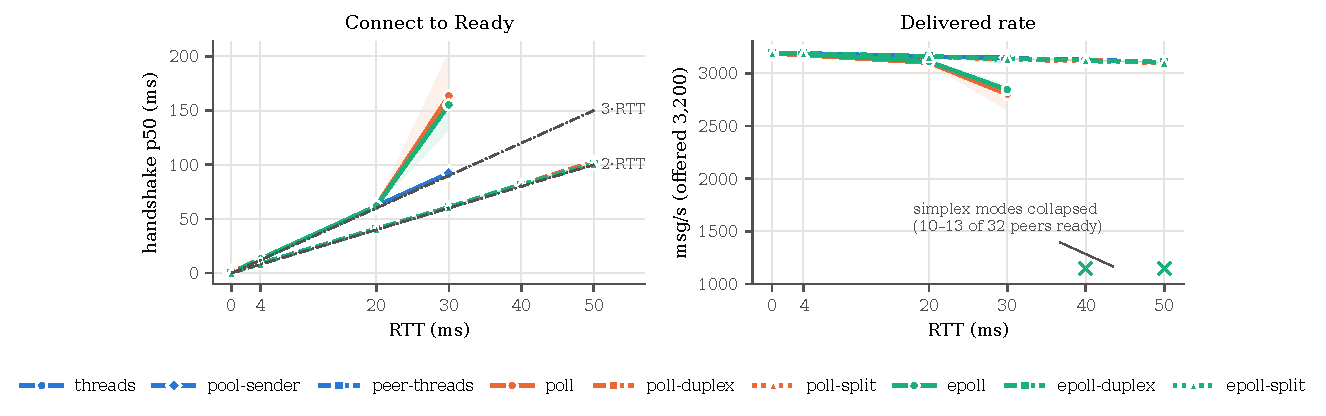
\includegraphics[width=\linewidth]{s6a_wan_churn}
\caption{S6a. Left: handshake p50 against RTT, with 2\,RTT and 3\,RTT guides. Right:
         delivered rate. Crosses mark the simplex cells that collapsed and were
         excluded as degraded.}
\label{fig:s6a}
\end{figure}

\finding{A handshake costs 3\,RTT in simplex and 2\,RTT in duplex.} At 20\,ms RTT the
simplex modes take 62\,ms to become ready and the duplex modes 41\,ms. At 50\,ms the
duplex modes take about 102\,ms (Figure~\ref{fig:s6a}).

\finding{The simplex collapse is a saturation cliff.} In every simplex mode, the
dial-back is a blocking \code{connect()} on the single sender thread. A churn event
costs that thread about two connects, so about $2\cdot\mathrm{RTT}$ of service time.
Its utilisation is $\rho = \mathrm{churn}\times 2\cdot\mathrm{RTT}$:
\begin{itemize}
  \item at 20\,ms, $\rho = 0.64$: stable, although the initial burst of 32 serialised
        connects gives a handshake p99 of 654\,ms;
  \item at 30\,ms, $\rho = 0.96$: \mode{poll} and \mode{epoll} degrade (2.8k msg/s,
        p50 about 100\,ms), while \mode{threads} and \mode{pool-sender} still hold;
  \item at 40 and 50\,ms, $\rho > 1$: all four simplex modes collapse. Only 10--13 of
        32 peers are ready, and the gates exclude all 24 cells.
\end{itemize}
The duplex modes never dial back and stay at about 3.1k msg/s throughout.

S6c repeats RTT 50\,ms with the churn halved to 8/s ($\rho = 0.8$). The simplex modes
recover to 3.0k msg/s, with a handshake p50 of 155\,ms (3\,RTT) and a p99 of 1.7\,s.
The collapse is therefore a cliff at $\rho = 1$, not a gradual slope.

\finding{What causes the cliff, and what defines it.} The sender's 100\,ms retry
sleep, which sets the tail in S4, plays no part here. The collapsed cells record only
1--4 failed sends per run, which is at most 0.4\,s of sleep in a 25\,s run. The cause
is the serial, blocking dial-back. The \emph{sharpness} of the cliff, however, also
comes from how the benchmark defines churn and validity:
\begin{itemize}
  \item Churn is open loop and always closes a \emph{ready} peer
        (Section~\ref{sec:gen}). Once the sender completes handshakes more slowly
        than churn removes ready peers, the set of ready peers drains and the backlog
        of dial-backs only grows. In the collapsed cells, only 278--341 of the 400
        scheduled churn events found a ready peer to close, the handshake p50 grew to
        2.6--3.2\,s, and the generator received no echoes in the window.
  \item A cell is excluded once fewer than 90\% of its peers are ready at the end.
\end{itemize}
A churn schedule that waits for each redial to finish, or a longer window, would
likely show the same overload as a gradual slowdown. The limit itself, one blocking
dial-back per churn event on one shared thread, belongs to the node. Where along that
curve a cell is called ``collapsed'' belongs to the benchmark.

\begin{table}[h]
\centering\small
\begin{tabular}{@{}lrrrrr@{}}
\tablebody{tables/s6b.tex}
\end{tabular}
\caption{S6b: msg/s at three node egress rates (16\,KiB messages, 4\,ms RTT), queued
         sends at 50\,Mbit/s, and handshake p50 at 1\,Gbit/s.}
\label{tab:s6b}
\end{table}

\finding{Behind a bottleneck, the link sets the pace.} In S6b every mode reaches the
same link-limited rate (Table~\ref{tab:s6b}), about 95\% of line rate. Writes queue as
designed: 4--5k queued sends at 50\,Mbit/s, and fewer than 60 at 1\,Gbit/s. Split and
duplex are identical within noise, so a separate write thread gains nothing when the
link is the limit. Simplex handshakes take about 78\,ms against 9\,ms, because the
dial-back's Ack queues behind data on the rate-limited node egress.

%-----------------------------------------------------------------------------
\subsection{S7: capped fan-in}

\begin{figure}[h]
\centering
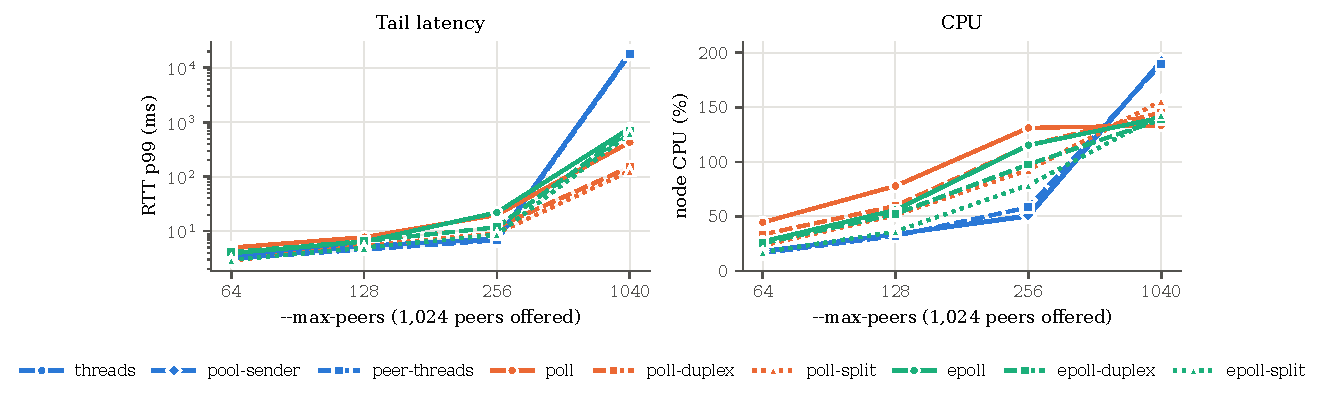
\includegraphics[width=\linewidth]{s7_capped}
\caption{S7. 1,024 peers offered against a node cap. 1040 is effectively uncapped.}
\label{fig:s7}
\end{figure}

\begin{table}[h]
\centering\small
\begin{tabular}{@{}lrrrrrr@{}}
\tablebody{tables/s7_256.tex}
\end{tabular}
\caption{S7 at \code{-{}-max-peers 256}.}
\label{tab:s7}
\end{table}

\finding{A cap turns collapse into shedding.} With a cap of 256
(Table~\ref{tab:s7}), \mode{threads} serves its 256 peers with no loss, a p99 of
7.1\,ms and 50\% CPU. Uncapped, it delivers 15.6k msg/s and loses 1.7\,M messages.
\mode{peer-threads} reaches a p99 of 6.8\,ms at 58\% CPU. In both, evictions equal
$1024 - \mathrm{cap}$ exactly. Capped \mode{epoll} uses 115\% CPU, the same as S1
\mode{epoll} at 256 peers (114\%). That is simply the cost of a single I/O thread
serving 256 peers (Section~\ref{sec:res-fanin}), not re-dial churn.

\textbf{The cap is not uniform across modes:}
\begin{itemize}
  \item the duplex and split pools hold \code{max\_peers}${}+16$ connections, so they
        serve 80, 144 and 272 peers;
  \item the dual pools hold $2\times$\code{max\_peers} connections, shared with
        dial-backs, so they serve the cap or one fewer;
  \item the thread modes serve exactly the cap.
\end{itemize}
Multiplexed prunes are also not counted as evictions. Modes must therefore be compared
by the number of peers they served, not by the nominal cap.

\section{Blocking calls, \texttt{poll} and \texttt{epoll} compared}
\label{sec:compare}

Section~\ref{sec:results} goes through the measurements one scenario at a time. This
section reads them the other way round. It takes the three ways a program can wait
for a socket and compares them across all scenarios: a blocking call on a thread of
its own, \code{poll(2)}, and \code{epoll(7)}.

\subsection{How each one waits}

\begin{description}
  \item[Blocking calls.] Each socket gets a thread that sits in \code{recv()} (or
        \code{send()}) until the call can complete. When data arrives, the kernel
        wakes exactly the thread that waits on that socket. No user-space code has to
        find out \emph{which} socket is ready, and the threads run on all cores at
        once. The price is a thread per socket: a stack, a scheduler entry, and one
        context switch per wake-up. A blocking call also waits as long as the peer
        lets it, which is why \mode{threads} sets a 500\,ms \code{SO\_SNDTIMEO} on
        sends and a 200\,ms timeout on reads.
  \item[\code{poll}.] One thread passes an array with every socket it watches to
        each call. The kernel checks every entry and the call returns the whole
        array, so a wait costs time proportional to the number of sockets, whether
        or not they are active. In this node, \code{receive()} returns one chunk
        per call, so every message read pays for one such scan
        (Section~\ref{sec:wrap-poll}).
  \item[\code{epoll}.] The interest list lives in the kernel. A socket is registered
        once with \code{epoll\_ctl}, the kernel puts it on a ready list when it
        becomes readable or writable, and \code{epoll\_wait} returns only the ready
        ones. A wait therefore costs time proportional to the number of
        \emph{ready} sockets. Other threads can change the interest list while the
        I/O thread is blocked in \code{epoll\_wait}, so no hand-off is needed. Both
        pools here are level-triggered.
\end{description}

\code{poll} and \code{epoll} need non-blocking sockets, and the program has to keep
its own buffer for a write that did not fit. It arms writability (\code{POLLOUT} or
\code{EPOLLOUT}) only while that buffer holds data. With blocking calls, the kernel
keeps the unsent bytes and the thread simply waits.

\subsection{\texttt{poll} against \texttt{epoll}}

Three pairs of modes differ only in the readiness API: \mode{poll}/\mode{epoll},
\mode{poll-duplex}/\mode{epoll-duplex} and \mode{poll-split}/\mode{epoll-split}.
Table~\ref{tab:cmp-poll-epoll} puts each pair side by side.

\begin{table}[h]
\centering\small
\begin{tabular}{@{}lcccccc@{}}
\tablebody{tables/cmp_poll_epoll.tex}
\end{tabular}
\caption{\code{poll} against \code{epoll} in each socket topology. Each cell gives
         the \code{poll} value, then the \code{epoll} value.}
\label{tab:cmp-poll-epoll}
\end{table}

\finding{With many sockets but few active ones, \code{epoll} is much cheaper.}
\begin{itemize}
  \item With 1,000 idle peers (S2), \code{poll} uses 65--100\% CPU and \code{epoll}
        10--17\%. The \code{epoll} variants cost about the same as with no idle peers
        at all.
  \item The \code{poll} p99 rises to 2.2--3.3\,ms, against about 1.0\,ms for
        \code{epoll}.
  \item The duplex and split modes have half as many sockets as simplex, and their
        \code{poll} cost is lower in proportion: 65--68\% against 100\%.
\end{itemize}
This is the per-call scan of the whole array, described above.

\finding{When most sockets are active, the difference shrinks.} At 256 active peers
(S1), \code{epoll} still uses less CPU in every topology (74--114\% against
87--132\%), but by 9--15\%, not by a factor of five. Most sockets are ready at every
wake-up, so \code{epoll} returns nearly as many entries as \code{poll} scans. With a
few sockets (S1 at 8 peers, S3, S5) the two are equal within a few percent of CPU,
and so is the latency.

\finding{Throughput does not depend on the readiness API.} In S5 and S6b the pairs
deliver the same rate within noise, with no consistent winner. Once the I/O thread is
busy reading and writing, the cost of finding the ready sockets is a small part of
its work. Behind a bottleneck link (S6b), \code{epoll} uses 8--14 percentage points less CPU for the
same rate.

\finding{At 1,024 busy peers, \code{poll} has the better tail.} This is the only
point where \code{poll} wins. Its p99 is 126--445\,ms, against 654--772\,ms for
\code{epoll}, at similar CPU. Section~\ref{sec:res-fanin} reports this as an
unexplained observation; the order in which each pool serves ready sockets is the
most likely cause.

\finding{Under churn, neither API decides the result.} In S4 both reach a p99 near or
above 100\,ms, set by the sender's retry sleep (Section~\ref{sec:res-churn}).

\subsection{Blocking calls against readiness multiplexing}

Table~\ref{tab:cmp-blocking} compares three modes at the same points:
\begin{itemize}
  \item \mode{threads}: blocking reads and blocking writes;
  \item \mode{pool-sender}: blocking reads, with writes made non-blocking through a
        pool;
  \item \mode{epoll-duplex}: one \code{epoll} thread for everything, the cheapest
        single-thread mode.
\end{itemize}

\begin{table}[h]
\centering\small
\setlength{\tabcolsep}{4pt}
\begin{tabular}{@{}lrrrrrrrrr@{}}
\tablebody{tables/cmp_blocking.tex}
\end{tabular}
\caption{Blocking calls against one \code{epoll} thread.}
\label{tab:cmp-blocking}
\end{table}

\finding{Blocking reads win up to a few hundred peers.} At 256 peers, the blocking
modes use 49\% CPU with a p99 of 7.1--7.2\,ms. \mode{epoll-duplex} needs 91\% for a
p99 of 10.7\,ms. With 4\,KiB messages (S5), the blocking modes deliver 109--113k
msg/s and \mode{epoll-duplex} 51k. There are two reasons:
\begin{itemize}
  \item the kernel wakes exactly the reader whose socket has data, so no time is
        spent finding it;
  \item the readers run on both cores, while one I/O thread can use only one.
\end{itemize}

\finding{Idle sockets cost blocking threads little CPU, but they cost memory.} With
1,000 idle peers, \mode{threads} matches \mode{epoll-duplex}: about 1.0\,ms p99 at
13--17\% CPU. Both do far better than \code{poll}. A thread blocked in \code{recv()}
uses no CPU. Here each idle reader still wakes every 200\,ms, when its
\code{SO\_RCVTIMEO} expires, to update its heartbeat for the watchdog. That shows as
11.1 thousand voluntary context switches per second, against 5.9 thousand with no
idle peers, but CPU only rises from 12\% to 17\%. But the node runs 1,016 threads instead of 8, and at 1,024 peers its
resident memory grows from 21\,MB to 280--291\,MB.

\finding{Too many active threads collapse.} At 1,024 active peers on two CPUs, the
blocking modes deliver 10--15k of the 102.4k msg/s offered, with RTTs of 18--20\,s.
They make 89--91 thousand voluntary context switches per second, against about 10
thousand for \mode{epoll-duplex}. \mode{epoll-duplex} delivers the whole load at
139\% CPU. A cap on peers (S7) prevents the collapse, but it also refuses peers.

\finding{Blocking writes on a shared thread are the real danger.} Blocking
\emph{reads} only ever stall their own thread. A blocking \emph{write} on the one
sender thread stalls every peer behind it: with four slow peers, \mode{threads}
reaches a p99 of 2.2\,s. \mode{pool-sender} keeps the same blocking reads but makes
writes non-blocking, and stays at 1.4\,ms. Blocking reads with non-blocking writes is
therefore the combination that worked best in this project, up to the thread limit.

\finding{Under churn, the blocking write behaves best.} \mode{threads} keeps a p99 of
4.6\,ms at 50 reconnects/s, while the non-blocking modes reach about 100\,ms. As
Section~\ref{sec:res-churn} explains, this comes from the sender's retry policy rather
than from blocking itself. A blocking \code{send()} to a socket that has just closed
still succeeds into the kernel buffer, so no retry sleep is triggered.

\finding{A blocking \code{connect()} remains in every mode.} Even the \code{poll}
and \code{epoll} modes dial with a blocking \code{connect()} on the sender thread.
That one blocking call causes the simplex collapse over a WAN (S6a). A fully
non-blocking design would also have to make \code{connect()} non-blocking and wait
for writability to learn when the connection is up.

\subsection{Summary}

\begin{table}[h]
\centering\small
\begin{tabularx}{\linewidth}{@{}>{\raggedright\arraybackslash}p{3.3cm}
    >{\raggedright\arraybackslash}X>{\raggedright\arraybackslash}X
    >{\raggedright\arraybackslash}X@{}}
\toprule
 & Blocking calls (thread per socket) & \code{poll} (one thread) & \code{epoll} (one thread) \\
\midrule
Cost of one wait & one context switch per wake-up & proportional to all sockets & proportional to ready sockets \\
Idle sockets & free in CPU, one thread each & every socket scanned on every call & free \\
Uses several cores & yes & no (one I/O thread) & no (one I/O thread) \\
Few active peers & cheapest, lowest latency & close to \code{epoll} & close to \code{poll} \\
1,024 active peers (2 CPUs) & collapses & full load & full load \\
Slow peer & stalls everyone if writes block & isolated & isolated \\
Code needed & simplest: the kernel buffers & non-blocking sockets, own write buffers & as \code{poll}, plus an epoll fd \\
\bottomrule
\end{tabularx}
\caption{Blocking calls, \code{poll} and \code{epoll} as measured in this project.}
\label{tab:cmp-summary}
\end{table}

Table~\ref{tab:cmp-summary} sums up. On a small node, blocking reads with non-blocking
writes were the simplest and the fastest, as long as the number of peers was capped
to what the cores could serve. Past that point, a readiness API is needed. Between
the two, \code{epoll} is never meaningfully worse than \code{poll} except in the
unexplained tail at 1,024 busy peers, and it is far better once many sockets are idle.

\section{Conclusions and final summary}
\label{sec:conclusions}

Every conclusion below rests on the measured run (Section~\ref{sec:method}) and on
the code it was built from. Each one was checked against the data. Claims that did not survive that
check are not included.

\subsection{Conclusions supported by the data}

\paragraph{C1. A second, simplex connection per peer is not worth it.}
\begin{itemize}
  \item \textbf{No throughput gain.} At 32\,B it is slower than duplex: \mode{poll}
        158k against 188k msg/s, \mode{epoll} 169k against 189k. At 4 and 64\,KiB the
        two shapes are within noise.
  \item \textbf{A longer handshake.} It costs 3\,RTT instead of 2: 62 against 41\,ms at
        20\,ms RTT, and a p50 of about 280 against 95\,ms at 1,024 peers.
  \item \textbf{An unreliable handshake under churn.} It collapses from 40\,ms RTT
        under 16 reconnects/s, and it slows behind a rate limit (78 against 9\,ms).
  \item \textbf{Twice the file descriptors.}
\end{itemize}
The collapse comes from the dial-back being a blocking \code{connect()} on the shared
sender thread, not from the retry sleep. How abruptly it appears is partly set by the
benchmark's open-loop churn and its 90\%-ready check (Section~\ref{sec:res-wan}). A non-blocking dial-back would remove the cliff, but not the extra
round trip or the extra connection.

\paragraph{C2. Separate read and write pollers pay off when the single I/O thread is
the bottleneck.} The trigger can be a high message rate, large messages or heavy
fan-in; any one is enough.
\begin{itemize}
  \item \textbf{Large messages, few peers:} with only 8 peers at 4\,KiB, the split
        modes deliver 46\% and 76\% more than duplex.
  \item \textbf{Fan-in:} at 256 peers, p99 is 8.0--8.4\,ms against about 10.6\,ms, at
        lower CPU. At 1,024 peers, p50 is 60 against 76\,ms (\mode{poll}) and 147
        against 159\,ms (\mode{epoll}).
  \item \textbf{No gain} when the link is the bottleneck (S6b) or the load is mostly
        idle (S2).
  \item \textbf{Worse under churn:} more failed sends.
\end{itemize}

\paragraph{C3. \mode{peer-threads} is reliable and fast, but needs a thread cap, and
its retry path is a limitation of the current implementation.}
\begin{itemize}
  \item \textbf{Reliable:} all 96 of its cells are valid. It stays healthy in S6a at
        40--50\,ms RTT, where simplex collapses.
  \item \textbf{Fast:} 203k msg/s at 32\,B and 16.2k at 64\,KiB. It has the best p99
        at 256 peers (6.8\,ms) and shields other peers from a slow reader.
  \item \textbf{Needs a cap:} at 1,024 peers on two CPUs it delivers only 20.8k of
        102k msg/s. Capped at 256, it serves those peers at a p99 of 6.8\,ms and
        58\% CPU.
  \item \textbf{Limitation:} its writes are already non-blocking, but retries are a
        100\,ms sleep on the shared \code{SenderWorker} thread, which stalls every
        peer. That cost 29--33 failures, and a p99 of 64--103\,ms, at churn 50.
        \code{open()} also does a blocking \code{connect()} on the same thread.
\end{itemize}
The retry and the dial belong on the peer's own owner thread: a deadline in its poll
loop rather than a sleep, and an asynchronous dial. The shared sender would then
become a dispatcher into per-peer queues. Two caveats remain: \mode{peer-threads}
uses two fds per peer, and its backpressure path was never exercised (S3).

\paragraph{Also established.}
\begin{itemize}
  \item Thread-per-connection collapses at 1,024 peers on two CPUs, and below that
        ceiling it is the cheapest mode.
  \item \code{poll} pays for every idle socket; \code{epoll} does not.
  \item Only a blocking sender lets one slow reader stall everyone.
  \item Under churn, tail latency is set by the shared sender's retry sleep, not by
        the concurrency model or by isolating descriptors.
\end{itemize}

\paragraph{Which mode to use.}
\begin{itemize}
  \item \textbf{Up to a few hundred peers on few cores:} a thread per peer with
        pooled writes (\mode{peer-threads}, \mode{pool-sender}), with
        \code{-{}-max-peers} sized to the cores.
  \item \textbf{Many or mostly idle peers:} \mode{epoll-duplex}, or
        \mode{epoll-split} for large messages or high rates.
  \item \textbf{Churn over a WAN:} always duplex.
\end{itemize}

\subsection{Limitations and open observations}

\begin{itemize}
  \item The measurements come from one WSL2 host, count CPU for the node only, and
        give the node two CPUs, which sets where the thread ceiling falls.
  \item Two observations remain unexplained:
        \begin{itemize}
          \item why the poll-based duplex and split modes beat \code{epoll} at 1,024
                peers;
          \item why the duplex shapes never queued writes in S3.
        \end{itemize}
  \item The peer cap is not uniform across modes (S7).
  \item Open-loop churn turns sender overload into an abrupt exclusion rather than a
        gradual slowdown (S6a).
\end{itemize}

\subsection{Final summary: a hypothesis for a combined design}

The tested results above bracket a design we did not build or measure. We state it as
a hypothesis.

\paragraph{Proposal.} Keep the ownership model of \mode{peer-threads}, in which one
thread owns its sockets, reads them and reports their end. But give each owner thread
a \emph{small pool of peers} instead of one, and add a balancing policy. This is an
M:N reactor~\cite{reactor} that sits between the two extremes we measured: one peer
per pool (\mode{peer-threads}) and every peer in one pool (\mode{*-duplex} and
\mode{*-split}). Candidate balancing policies:
\begin{itemize}
  \item uniform: assign each new peer to the least-loaded pool;
  \item separate pools for peers that send large messages and peers that send small
        ones;
  \item separate pools for unreliable or churning peers.
\end{itemize}

\paragraph{Why the data makes it plausible.}
\begin{itemize}
  \item \textbf{No CPU starvation.} A bounded number of threads avoids the collapse
        at 1,024 peers; the single-poller modes served 1,024 peers at about 140\% CPU.
  \item \textbf{Uses the cores.} One I/O thread plateaus at about 122--144\% CPU in
        S5, while the thread modes reach 170--180\%. Roughly one pool per core could
        reach the same.
  \item \textbf{\code{poll} is cheap for small pools.} Its cost grows with the number
        of descriptors (S2), and the poll-based duplex and split modes had the best
        fan-in latency.
  \item \textbf{Fewer descriptors.} One eventfd per pool instead of one per peer gives
        about \emph{peers + pools}.
\end{itemize}

\paragraph{Preconditions and risks.}
\begin{itemize}
  \item \textbf{The sender's policy has to move into the pool loops.} Retries and
        dials (C3) must become timers there. Otherwise the S4 tail and the S6a cliff
        remain. A plain sleep inside a pool would stall every peer in that pool.
  \item \textbf{Place peers once.} A peer should be assigned when it attaches, without
        migration at first. Moving a live connection means handing over its fd and
        its \code{FrameChannel}.
  \item \textbf{Some isolation policies lack evidence.} Isolating large-message peers
        is motivated by S5 but untested. Isolating slow readers showed no clear need,
        since pooled writes did not stall in S3.
\end{itemize}
Evaluating it would mean sweeping the pool size (1, 8, 32, all) with about one pool
per core, over S1, S4 and S5, under one capacity rule for every mode.

\paragraph{Other directions.} A completion-based backend
(\code{io\_uring}~\cite{iouring}) behind the same \code{IoStack}, and QUIC~\cite{quic},
which is duplex and multiplexed by design.


\appendix
\section{Reproduction}
\label{app:repro}

\paragraph{The measured run.} All results in this report come from the directory
\code{results-0294f37}, produced by a clean Release build of commit \code{0294f37} on
the branch \code{io-variants}. The repository contains, for every cell and repetition,
the metadata (\code{rep*.meta.json}), the generator's result (\code{rep*.stress.json})
and the node's metrics (\code{rep*.metrics.jsonl}), together with \code{summary.csv}
and \code{report.html}. The node and generator logs are not committed.

\paragraph{Build and run.}
\begin{verbatim}
cmake -B build -S . -DCMAKE_BUILD_TYPE=Release && cmake --build build -j
scripts/run_matrix.py --app build/app --stressgen build/stressgen \
    --out results-<commit> --reps 3
scripts/analyze.py results-<commit>      # summary.csv, report.html
\end{verbatim}

\paragraph{Notes.}
\begin{itemize}
  \item The working tree must be clean, so every cell's build stamp names an exact
        commit.
  \item The node runs on CPUs 0--1 and the generator on CPUs 4--7.
  \item An interrupted run resumes when the same command is run again: cells that
        completed are kept and failed ones are retried. It refuses to mix builds.
\end{itemize}

\paragraph{Figures and tables.} Every figure and table in Section~\ref{sec:results}
is generated from \code{results-0294f37} by the script \code{make\_figures.py} in
the directory \code{report/visualisation-scripts}. The handshake diagrams
(Figure~\ref{fig:handshake}) are PlantUML sources in the same directory, rendered by
\code{make\_handshake.sh}.

\section{Test suite}

\begin{itemize}
  \item One unit-test executable per component: queue, wire format, sockets and pools,
        \code{TxPoller}, store, sender, workers, rendering, metrics, \code{stressgen},
        \code{peer-threads} and others.
  \item An end-to-end script that runs two headless nodes in every mode.
  \item Tests for the analysis script.
  \item A normal \code{ctest -j8} passes 26 of 26 tests.
\end{itemize}

\paragraph{Parallel load.} Running six to eight copies of the network-heavy tests at
once still fails about 2\% of runs, because fixed deadlines in the two-node checks
expire under that artificial load (see also Section~\ref{sec:lessons}).

\section{All results}
\label{app:full}

Tables~\ref{tab:full-S1}--\ref{tab:full-S7} list every swept value and every mode of
every scenario. Each value is the median over the valid repetitions; ``valid'' gives
how many of the three repetitions passed the validity checks, and a cell with no
valid repetition shows dashes. Columns:
\begin{itemize}
  \item \textbf{msg/s}: echoed messages per second; \textbf{lost}: messages sent in
        the window and never echoed;
  \item \textbf{p50}, \textbf{p99}, \textbf{p99.9}: round-trip time in ms;
  \item \textbf{CPU \%}: node CPU usage (Equation~\ref{eq:cpu}); \textbf{vol./s} and
        \textbf{invol./s}: voluntary and involuntary context switches per second;
  \item \textbf{thr.} and \textbf{fds}: the node's peak thread and descriptor counts;
  \item \textbf{ready}: peers that completed the handshake; \textbf{hs p50}: median
        handshake time in ms;
  \item \textbf{queued}: sends that had to be queued because the socket's transmit
        buffer was full; \textbf{evict.}: peers evicted by the cap.
\end{itemize}

\begin{landscape}
\scriptsize
\setlength{\tabcolsep}{4pt}
\setlength{\LTcapwidth}{\linewidth}
\begin{longtable}{@{}llrrrrrrrrrrrrrrr@{}}
\caption{S1 (fan-in): all results.}\label{tab:full-S1}\\
\toprule
peers & Variant & valid & msg/s & lost & p50 & p99 & p99.9 & CPU \% & vol./s & invol./s & thr. & fds & ready & hs p50 & queued & evict. \\
\midrule
\endfirsthead
\toprule
peers & Variant & valid & msg/s & lost & p50 & p99 & p99.9 & CPU \% & vol./s & invol./s & thr. & fds & ready & hs p50 & queued & evict. \\
\midrule
\endhead
\bottomrule
\endfoot
1 & \texttt{threads} & 3/3 & 100 & 0 & 0.7 & 1.8 & 2.5 & 2 & 331 & 0 & 9 & 8 & 1 & 1.9 & 0 & 0 \\
 & \texttt{pool-sender} & 3/3 & 100 & 0 & 0.7 & 1.8 & 2.6 & 2 & 335 & 0 & 10 & 9 & 1 & 2.5 & 0 & 0 \\
 & \texttt{peer-threads} & 3/3 & 100 & 0 & 0.7 & 2.1 & 3.1 & 2 & 335 & 0 & 9 & 8 & 1 & 1.4 & 0 & 0 \\
 & \texttt{poll} & 3/3 & 100 & 0 & 0.8 & 1.6 & 2.2 & 2 & 324 & 0 & 8 & 9 & 1 & 2.2 & 0 & 0 \\
 & \texttt{poll-duplex} & 3/3 & 100 & 0 & 0.7 & 1.8 & 2.7 & 2 & 325 & 0 & 8 & 8 & 1 & 1.5 & 0 & 0 \\
 & \texttt{poll-split} & 3/3 & 100 & 0 & 0.7 & 2.2 & 3.2 & 2 & 325 & 0 & 9 & 9 & 1 & 2.2 & 0 & 0 \\
 & \texttt{epoll} & 3/3 & 100 & 0 & 0.7 & 1.9 & 2.9 & 2 & 325 & 0 & 8 & 10 & 1 & 2.0 & 0 & 0 \\
 & \texttt{epoll-duplex} & 3/3 & 100 & 0 & 0.6 & 1.9 & 2.9 & 2 & 325 & 0 & 8 & 9 & 1 & 2.1 & 0 & 0 \\
 & \texttt{epoll-split} & 3/3 & 100 & 0 & 0.7 & 1.9 & 2.8 & 2 & 325 & 0 & 9 & 11 & 1 & 1.8 & 0 & 0 \\
\midrule
8 & \texttt{threads} & 3/3 & 800 & 0 & 0.9 & 1.7 & 2.6 & 4 & 1{,}382 & 55 & 16 & 22 & 8 & 5.1 & 0 & 0 \\
 & \texttt{pool-sender} & 3/3 & 800 & 0 & 0.9 & 1.6 & 2.4 & 4 & 1{,}358 & 60 & 17 & 23 & 8 & 4.6 & 0 & 0 \\
 & \texttt{peer-threads} & 3/3 & 800 & 0 & 1.0 & 2.0 & 2.9 & 3 & 1{,}383 & 53 & 16 & 22 & 8 & 2.9 & 0 & 0 \\
 & \texttt{poll} & 3/3 & 800 & 0 & 1.0 & 1.7 & 2.4 & 5 & 817 & 2 & 8 & 23 & 8 & 4.1 & 0 & 0 \\
 & \texttt{poll-duplex} & 3/3 & 800 & 0 & 0.9 & 1.4 & 2.8 & 4 & 665 & 1 & 8 & 15 & 8 & 2.2 & 0 & 0 \\
 & \texttt{poll-split} & 3/3 & 800 & 0 & 1.0 & 2.2 & 3.4 & 3 & 493 & 3 & 9 & 16 & 8 & 2.2 & 0 & 0 \\
 & \texttt{epoll} & 3/3 & 800 & 0 & 1.0 & 1.7 & 2.4 & 4 & 757 & 1 & 8 & 24 & 8 & 5.0 & 0 & 0 \\
 & \texttt{epoll-duplex} & 3/3 & 800 & 0 & 1.0 & 2.2 & 3.0 & 3 & 542 & 0 & 8 & 16 & 8 & 2.9 & 0 & 0 \\
 & \texttt{epoll-split} & 3/3 & 800 & 0 & 1.0 & 2.2 & 3.3 & 3 & 507 & 3 & 9 & 18 & 8 & 1.8 & 0 & 0 \\
\midrule
64 & \texttt{threads} & 3/3 & 6{,}400 & 0 & 1.8 & 3.8 & 5.5 & 18 & 8{,}409 & 690 & 72 & 134 & 64 & 51.4 & 0 & 0 \\
 & \texttt{pool-sender} & 3/3 & 6{,}400 & 0 & 1.9 & 3.9 & 5.4 & 19 & 8{,}247 & 639 & 73 & 135 & 64 & 46.1 & 0 & 0 \\
 & \texttt{peer-threads} & 3/3 & 6{,}400 & 0 & 1.7 & 3.2 & 3.9 & 17 & 9{,}036 & 786 & 72 & 134 & 64 & 24.6 & 0 & 0 \\
 & \texttt{poll} & 3/3 & 6{,}400 & 0 & 2.4 & 4.5 & 5.2 & 35 & 6{,}672 & 150 & 8 & 135 & 64 & 48.2 & 0 & 0 \\
 & \texttt{poll-duplex} & 3/3 & 6{,}400 & 0 & 2.1 & 3.7 & 4.5 & 24 & 5{,}206 & 146 & 8 & 71 & 64 & 6.7 & 0 & 0 \\
 & \texttt{poll-split} & 3/3 & 6{,}400 & 0 & 1.7 & 3.2 & 4.7 & 20 & 3{,}926 & 1{,}134 & 9 & 72 & 64 & 5.9 & 0 & 0 \\
 & \texttt{epoll} & 3/3 & 6{,}400 & 0 & 2.2 & 3.9 & 4.8 & 26 & 4{,}774 & 102 & 8 & 136 & 64 & 50.3 & 0 & 0 \\
 & \texttt{epoll-duplex} & 3/3 & 6{,}400 & 0 & 2.0 & 3.6 & 4.3 & 19 & 4{,}381 & 107 & 8 & 72 & 64 & 5.6 & 0 & 0 \\
 & \texttt{epoll-split} & 3/3 & 6{,}400 & 0 & 1.7 & 3.0 & 3.7 & 14 & 2{,}472 & 468 & 9 & 74 & 64 & 4.7 & 0 & 0 \\
\midrule
256 & \texttt{threads} & 3/3 & 25{,}600 & 0 & 4.1 & 7.2 & 8.7 & 49 & 28{,}529 & 1{,}308 & 264 & 518 & 256 & 151.0 & 0 & 0 \\
 & \texttt{pool-sender} & 3/3 & 25{,}600 & 0 & 4.0 & 7.1 & 8.9 & 49 & 28{,}615 & 1{,}315 & 265 & 519 & 256 & 142.6 & 0 & 0 \\
 & \texttt{peer-threads} & 3/3 & 25{,}600 & 0 & 3.9 & 6.8 & 9.7 & 54 & 29{,}814 & 1{,}592 & 264 & 518 & 256 & 96.5 & 0 & 0 \\
 & \texttt{poll} & 3/3 & 25{,}600 & 0 & 11.5 & 22.5 & 28.3 & 132 & 25{,}314 & 221 & 8 & 519 & 256 & 117.4 & 0 & 0 \\
 & \texttt{poll-duplex} & 3/3 & 25{,}600 & 0 & 4.8 & 10.5 & 13.9 & 100 & 37{,}505 & 870 & 8 & 263 & 256 & 51.4 & 0 & 0 \\
 & \texttt{poll-split} & 3/3 & 25{,}600 & 0 & 3.7 & 8.4 & 11.0 & 87 & 25{,}834 & 4{,}772 & 9 & 264 & 256 & 41.9 & 0 & 0 \\
 & \texttt{epoll} & 3/3 & 25{,}600 & 0 & 6.3 & 19.4 & 41.9 & 114 & 32{,}103 & 1{,}008 & 8 & 520 & 256 & 115.3 & 0 & 0 \\
 & \texttt{epoll-duplex} & 3/3 & 25{,}600 & 0 & 5.4 & 10.7 & 18.4 & 91 & 32{,}043 & 994 & 8 & 264 & 256 & 67.1 & 0 & 0 \\
 & \texttt{epoll-split} & 3/3 & 25{,}600 & 0 & 4.1 & 8.0 & 8.9 & 74 & 18{,}500 & 3{,}928 & 9 & 266 & 256 & 55.6 & 0 & 0 \\
\midrule
1{,}024 & \texttt{threads} & 3/3 & 15{,}114 & 1{,}745{,}710 & 18{,}253.6 & 18{,}643.5 & 18{,}643.5 & 193 & 88{,}807 & 2{,}938 & 1{,}032 & 2{,}054 & 1{,}024 & 293.6 & 0 & 0 \\
 & \texttt{pool-sender} & 3/3 & 10{,}370 & 1{,}840{,}600 & 19{,}327.4 & 19{,}503.3 & 19{,}503.3 & 192 & 91{,}182 & 2{,}820 & 1{,}033 & 2{,}055 & 1{,}024 & 310.4 & 0 & 0 \\
 & \texttt{peer-threads} & 3/3 & 20{,}794 & 1{,}632{,}110 & 16{,}374.6 & 17{,}551.8 & 17{,}551.8 & 190 & 106{,}962 & 3{,}968 & 1{,}032 & 2{,}054 & 1{,}024 & 159.4 & 0 & 0 \\
 & \texttt{poll} & 3/3 & 102{,}400 & 0 & 209.7 & 444.6 & 503.3 & 133 & 6{,}315 & 603 & 8 & 2{,}055 & 1{,}024 & 285.2 & 0 & 0 \\
 & \texttt{poll-duplex} & 3/3 & 102{,}400 & 0 & 75.5 & 167.8 & 247.5 & 145 & 15{,}858 & 745 & 8 & 1{,}031 & 1{,}024 & 94.4 & 0 & 0 \\
 & \texttt{poll-split} & 3/3 & 102{,}400 & 0 & 59.8 & 125.8 & 155.2 & 156 & 15{,}508 & 2{,}340 & 9 & 1{,}032 & 1{,}024 & 111.1 & 0 & 0 \\
 & \texttt{epoll} & 3/3 & 102{,}400 & 0 & 176.2 & 771.8 & 1{,}107.3 & 140 & 9{,}615 & 577 & 8 & 2{,}056 & 1{,}024 & 276.8 & 0 & 0 \\
 & \texttt{epoll-duplex} & 3/3 & 102{,}400 & 0 & 159.4 & 721.4 & 1{,}023.4 & 139 & 10{,}056 & 504 & 8 & 1{,}032 & 1{,}024 & 98.6 & 0 & 0 \\
 & \texttt{epoll-split} & 3/3 & 102{,}400 & 0 & 146.8 & 654.3 & 973.1 & 144 & 9{,}968 & 1{,}137 & 9 & 1{,}034 & 1{,}024 & 86.0 & 0 & 0 \\
\end{longtable}

\begin{longtable}{@{}llrrrrrrrrrrrrrrr@{}}
\caption{S2 (idle connections): all results.}\label{tab:full-S2}\\
\toprule
idle\_peers & Variant & valid & msg/s & lost & p50 & p99 & p99.9 & CPU \% & vol./s & invol./s & thr. & fds & ready & hs p50 & queued & evict. \\
\midrule
\endfirsthead
\toprule
idle\_peers & Variant & valid & msg/s & lost & p50 & p99 & p99.9 & CPU \% & vol./s & invol./s & thr. & fds & ready & hs p50 & queued & evict. \\
\midrule
\endhead
\bottomrule
\endfoot
0 & \texttt{threads} & 3/3 & 4{,}000 & 0 & 0.6 & 0.9 & 1.1 & 12 & 5{,}866 & 127 & 16 & 22 & 8 & 4.5 & 0 & 0 \\
 & \texttt{pool-sender} & 3/3 & 4{,}000 & 0 & 0.6 & 0.9 & 1.1 & 13 & 6{,}180 & 186 & 17 & 23 & 8 & 4.5 & 0 & 0 \\
 & \texttt{peer-threads} & 3/3 & 4{,}000 & 0 & 0.6 & 1.0 & 1.7 & 12 & 6{,}208 & 229 & 16 & 22 & 8 & 2.3 & 0 & 0 \\
 & \texttt{poll} & 3/3 & 4{,}000 & 0 & 0.7 & 1.0 & 1.3 & 19 & 4{,}314 & 8 & 8 & 23 & 8 & 3.7 & 0 & 0 \\
 & \texttt{poll-duplex} & 3/3 & 4{,}000 & 0 & 0.7 & 1.0 & 1.4 & 12 & 2{,}738 & 3 & 8 & 15 & 8 & 1.9 & 0 & 0 \\
 & \texttt{poll-split} & 3/3 & 4{,}000 & 0 & 0.7 & 0.9 & 1.3 & 10 & 2{,}103 & 26 & 9 & 16 & 8 & 1.6 & 0 & 0 \\
 & \texttt{epoll} & 3/3 & 4{,}000 & 0 & 0.6 & 1.0 & 1.2 & 17 & 3{,}936 & 6 & 8 & 24 & 8 & 4.5 & 0 & 0 \\
 & \texttt{epoll-duplex} & 3/3 & 4{,}000 & 0 & 0.7 & 1.0 & 1.6 & 13 & 2{,}899 & 2 & 8 & 16 & 8 & 2.4 & 0 & 0 \\
 & \texttt{epoll-split} & 3/3 & 4{,}000 & 0 & 0.7 & 1.0 & 1.4 & 11 & 2{,}421 & 13 & 9 & 18 & 8 & 2.1 & 0 & 0 \\
\midrule
100 & \texttt{threads} & 3/3 & 4{,}000 & 0 & 0.6 & 0.9 & 1.1 & 13 & 6{,}411 & 152 & 116 & 222 & 108 & 66.1 & 0 & 0 \\
 & \texttt{pool-sender} & 3/3 & 4{,}000 & 0 & 0.6 & 0.9 & 1.1 & 14 & 6{,}511 & 157 & 117 & 223 & 108 & 88.1 & 0 & 0 \\
 & \texttt{peer-threads} & 3/3 & 4{,}000 & 0 & 0.7 & 1.0 & 1.6 & 12 & 6{,}404 & 166 & 116 & 222 & 108 & 36.7 & 0 & 0 \\
 & \texttt{poll} & 3/3 & 4{,}000 & 0 & 0.7 & 1.2 & 1.5 & 35 & 6{,}962 & 78 & 8 & 223 & 108 & 81.8 & 0 & 0 \\
 & \texttt{poll-duplex} & 3/3 & 4{,}000 & 0 & 0.7 & 1.1 & 1.5 & 23 & 5{,}364 & 15 & 8 & 115 & 108 & 6.7 & 0 & 0 \\
 & \texttt{poll-split} & 3/3 & 4{,}000 & 0 & 0.7 & 1.0 & 1.4 & 20 & 5{,}230 & 415 & 9 & 116 & 108 & 8.3 & 0 & 0 \\
 & \texttt{epoll} & 3/3 & 4{,}000 & 0 & 0.6 & 1.0 & 1.3 & 18 & 3{,}963 & 5 & 8 & 224 & 108 & 71.3 & 0 & 0 \\
 & \texttt{epoll-duplex} & 3/3 & 4{,}000 & 0 & 0.7 & 1.0 & 1.8 & 13 & 2{,}909 & 2 & 8 & 116 & 108 & 8.3 & 0 & 0 \\
 & \texttt{epoll-split} & 3/3 & 4{,}000 & 0 & 0.7 & 1.0 & 1.5 & 10 & 1{,}999 & 9 & 9 & 118 & 108 & 8.4 & 0 & 0 \\
\midrule
300 & \texttt{threads} & 3/3 & 4{,}000 & 0 & 0.6 & 0.9 & 1.3 & 15 & 7{,}579 & 192 & 316 & 622 & 308 & 142.6 & 0 & 0 \\
 & \texttt{pool-sender} & 3/3 & 4{,}000 & 0 & 0.6 & 0.9 & 1.2 & 15 & 7{,}632 & 193 & 317 & 623 & 308 & 132.1 & 0 & 0 \\
 & \texttt{peer-threads} & 3/3 & 4{,}000 & 0 & 0.7 & 1.0 & 1.8 & 13 & 7{,}235 & 188 & 316 & 622 & 308 & 92.3 & 0 & 0 \\
 & \texttt{poll} & 3/3 & 4{,}000 & 0 & 0.8 & 1.4 & 2.2 & 51 & 8{,}096 & 11 & 8 & 623 & 308 & 142.6 & 0 & 0 \\
 & \texttt{poll-duplex} & 3/3 & 4{,}000 & 0 & 0.8 & 1.3 & 2.0 & 35 & 7{,}396 & 54 & 8 & 315 & 308 & 53.5 & 0 & 0 \\
 & \texttt{poll-split} & 3/3 & 4{,}000 & 0 & 0.8 & 1.1 & 1.8 & 34 & 6{,}609 & 116 & 9 & 316 & 308 & 62.9 & 0 & 0 \\
 & \texttt{epoll} & 3/3 & 4{,}000 & 0 & 0.6 & 1.0 & 1.3 & 18 & 3{,}966 & 8 & 8 & 624 & 308 & 134.2 & 0 & 0 \\
 & \texttt{epoll-duplex} & 3/3 & 4{,}000 & 0 & 0.6 & 1.0 & 1.7 & 13 & 2{,}888 & 3 & 8 & 316 & 308 & 55.6 & 0 & 0 \\
 & \texttt{epoll-split} & 3/3 & 4{,}000 & 0 & 0.6 & 1.0 & 1.6 & 10 & 2{,}044 & 15 & 9 & 318 & 308 & 54.5 & 0 & 0 \\
\midrule
1{,}000 & \texttt{threads} & 3/3 & 4{,}000 & 0 & 0.6 & 1.0 & 2.2 & 17 & 11{,}074 & 273 & 1{,}016 & 2{,}022 & 1{,}008 & 318.8 & 0 & 0 \\
 & \texttt{pool-sender} & 3/3 & 4{,}000 & 0 & 0.6 & 1.0 & 1.9 & 17 & 10{,}975 & 238 & 1{,}017 & 2{,}023 & 1{,}008 & 318.8 & 0 & 0 \\
 & \texttt{peer-threads} & 3/3 & 4{,}000 & 0 & 0.6 & 1.0 & 2.4 & 17 & 10{,}320 & 265 & 1{,}016 & 2{,}022 & 1{,}008 & 138.4 & 0 & 0 \\
 & \texttt{poll} & 3/3 & 4{,}000 & 0 & 1.4 & 3.3 & 4.8 & 100 & 7{,}215 & 12 & 8 & 2{,}023 & 1{,}008 & 268.4 & 0 & 0 \\
 & \texttt{poll-duplex} & 3/3 & 4{,}000 & 0 & 1.0 & 2.2 & 3.9 & 68 & 8{,}172 & 3 & 8 & 1{,}015 & 1{,}008 & 100.7 & 0 & 0 \\
 & \texttt{poll-split} & 3/3 & 4{,}000 & 0 & 0.9 & 2.2 & 3.4 & 65 & 8{,}114 & 9 & 9 & 1{,}016 & 1{,}008 & 90.2 & 0 & 0 \\
 & \texttt{epoll} & 3/3 & 4{,}000 & 0 & 0.6 & 1.0 & 2.7 & 17 & 4{,}028 & 6 & 8 & 2{,}024 & 1{,}008 & 276.8 & 0 & 0 \\
 & \texttt{epoll-duplex} & 3/3 & 4{,}000 & 0 & 0.7 & 1.1 & 2.8 & 13 & 2{,}906 & 2 & 8 & 1{,}016 & 1{,}008 & 83.9 & 0 & 0 \\
 & \texttt{epoll-split} & 3/3 & 4{,}000 & 0 & 0.6 & 1.0 & 1.9 & 10 & 1{,}987 & 8 & 9 & 1{,}018 & 1{,}008 & 86.0 & 0 & 0 \\
\end{longtable}

\begin{longtable}{@{}llrrrrrrrrrrrrrrr@{}}
\caption{S3 (slow consumers): all results.}\label{tab:full-S3}\\
\toprule
slow\_peers & Variant & valid & msg/s & lost & p50 & p99 & p99.9 & CPU \% & vol./s & invol./s & thr. & fds & ready & hs p50 & queued & evict. \\
\midrule
\endfirsthead
\toprule
slow\_peers & Variant & valid & msg/s & lost & p50 & p99 & p99.9 & CPU \% & vol./s & invol./s & thr. & fds & ready & hs p50 & queued & evict. \\
\midrule
\endhead
\bottomrule
\endfoot
0 & \texttt{threads} & 3/3 & 3{,}200 & 0 & 0.8 & 1.3 & 1.6 & 10 & 4{,}641 & 258 & 24 & 38 & 16 & 6.9 & 0 & 0 \\
 & \texttt{pool-sender} & 3/3 & 3{,}200 & 0 & 0.8 & 1.4 & 1.8 & 10 & 4{,}583 & 220 & 25 & 39 & 16 & 7.7 & 0 & 0 \\
 & \texttt{peer-threads} & 3/3 & 3{,}200 & 0 & 1.0 & 1.5 & 2.2 & 9 & 4{,}527 & 221 & 24 & 38 & 16 & 3.9 & 0 & 0 \\
 & \texttt{poll} & 3/3 & 3{,}200 & 0 & 1.0 & 1.5 & 2.0 & 14 & 2{,}919 & 11 & 8 & 39 & 16 & 8.1 & 0 & 0 \\
 & \texttt{poll-duplex} & 3/3 & 3{,}200 & 0 & 0.9 & 1.5 & 2.0 & 12 & 2{,}591 & 10 & 8 & 23 & 16 & 2.4 & 0 & 0 \\
 & \texttt{poll-split} & 3/3 & 3{,}200 & 0 & 0.9 & 1.4 & 2.2 & 9 & 1{,}422 & 70 & 9 & 24 & 16 & 2.8 & 0 & 0 \\
 & \texttt{epoll} & 3/3 & 3{,}200 & 0 & 0.9 & 1.5 & 2.0 & 13 & 2{,}638 & 12 & 8 & 40 & 16 & 6.8 & 0 & 0 \\
 & \texttt{epoll-duplex} & 3/3 & 3{,}200 & 0 & 1.0 & 1.5 & 2.0 & 10 & 2{,}351 & 8 & 8 & 24 & 16 & 2.5 & 0 & 0 \\
 & \texttt{epoll-split} & 3/3 & 3{,}200 & 0 & 0.9 & 1.4 & 2.0 & 8 & 1{,}393 & 43 & 9 & 26 & 16 & 2.7 & 0 & 0 \\
\midrule
1 & \texttt{threads} & 3/3 & 3{,}200 & 0 & 0.9 & 419.4 & 604.0 & 10 & 4{,}816 & 235 & 25 & 40 & 17 & 8.4 & 0 & 0 \\
 & \texttt{pool-sender} & 3/3 & 3{,}200 & 0 & 0.8 & 1.3 & 1.7 & 11 & 5{,}099 & 278 & 26 & 41 & 17 & 11.3 & 2{,}045 & 0 \\
 & \texttt{peer-threads} & 3/3 & 3{,}200 & 0 & 0.9 & 1.4 & 2.0 & 9 & 4{,}821 & 285 & 25 & 40 & 17 & 3.2 & 0 & 0 \\
 & \texttt{poll} & 3/3 & 3{,}200 & 0 & 1.0 & 1.5 & 1.9 & 16 & 3{,}294 & 17 & 8 & 41 & 17 & 8.1 & 2{,}046 & 0 \\
 & \texttt{poll-duplex} & 3/3 & 3{,}200 & 0 & 0.9 & 1.5 & 2.0 & 11 & 2{,}547 & 11 & 8 & 24 & 17 & 2.9 & 0 & 0 \\
 & \texttt{poll-split} & 3/3 & 3{,}200 & 0 & 0.9 & 1.4 & 2.6 & 8 & 1{,}413 & 68 & 9 & 25 & 17 & 2.2 & 0 & 0 \\
 & \texttt{epoll} & 3/3 & 3{,}200 & 0 & 0.9 & 1.5 & 1.8 & 13 & 2{,}700 & 10 & 8 & 42 & 17 & 11.0 & 2{,}046 & 0 \\
 & \texttt{epoll-duplex} & 3/3 & 3{,}200 & 0 & 0.9 & 1.5 & 2.0 & 11 & 2{,}277 & 6 & 8 & 25 & 17 & 2.9 & 0 & 0 \\
 & \texttt{epoll-split} & 3/3 & 3{,}200 & 0 & 0.9 & 1.5 & 1.9 & 8 & 1{,}301 & 34 & 9 & 27 & 17 & 3.9 & 0 & 0 \\
\midrule
4 & \texttt{threads} & 3/3 & 3{,}200 & 0 & 0.9 & 2{,}214.6 & 2{,}409.8 & 11 & 5{,}692 & 300 & 28 & 46 & 20 & 8.7 & 0 & 0 \\
 & \texttt{pool-sender} & 3/3 & 3{,}200 & 0 & 0.9 & 1.4 & 1.8 & 13 & 6{,}035 & 355 & 29 & 47 & 20 & 11.3 & 8{,}180 & 0 \\
 & \texttt{peer-threads} & 3/3 & 3{,}200 & 0 & 0.9 & 1.5 & 1.9 & 10 & 4{,}710 & 275 & 28 & 46 & 20 & 4.5 & 0 & 0 \\
 & \texttt{poll} & 3/3 & 3{,}200 & 0 & 1.0 & 1.6 & 1.9 & 19 & 3{,}918 & 31 & 8 & 47 & 20 & 8.9 & 8{,}184 & 0 \\
 & \texttt{poll-duplex} & 3/3 & 3{,}200 & 0 & 0.9 & 1.5 & 2.4 & 11 & 2{,}602 & 16 & 8 & 27 & 20 & 2.8 & 0 & 0 \\
 & \texttt{poll-split} & 3/3 & 3{,}200 & 0 & 0.9 & 1.5 & 2.2 & 8 & 1{,}344 & 85 & 9 & 28 & 20 & 3.3 & 0 & 0 \\
 & \texttt{epoll} & 3/3 & 3{,}200 & 0 & 1.0 & 1.6 & 1.9 & 16 & 3{,}427 & 68 & 8 & 48 & 20 & 9.4 & 8{,}178 & 0 \\
 & \texttt{epoll-duplex} & 3/3 & 3{,}200 & 0 & 1.0 & 1.5 & 1.9 & 11 & 2{,}379 & 9 & 8 & 28 & 20 & 2.6 & 0 & 0 \\
 & \texttt{epoll-split} & 3/3 & 3{,}200 & 0 & 0.9 & 1.5 & 2.1 & 7 & 1{,}224 & 30 & 9 & 30 & 20 & 3.1 & 0 & 0 \\
\end{longtable}

\begin{longtable}{@{}llrrrrrrrrrrrrrrr@{}}
\caption{S4 (churn): all results.}\label{tab:full-S4}\\
\toprule
churn & Variant & valid & msg/s & lost & p50 & p99 & p99.9 & CPU \% & vol./s & invol./s & thr. & fds & ready & hs p50 & queued & evict. \\
\midrule
\endfirsthead
\toprule
churn & Variant & valid & msg/s & lost & p50 & p99 & p99.9 & CPU \% & vol./s & invol./s & thr. & fds & ready & hs p50 & queued & evict. \\
\midrule
\endhead
\bottomrule
\endfoot
0 & \texttt{threads} & 3/3 & 3{,}200 & 0 & 2.2 & 4.0 & 5.4 & 10 & 4{,}104 & 290 & 72 & 134 & 64 & 55.6 & 0 & 0 \\
 & \texttt{pool-sender} & 3/3 & 3{,}200 & 0 & 2.3 & 3.9 & 4.8 & 10 & 4{,}107 & 290 & 73 & 135 & 64 & 53.5 & 0 & 0 \\
 & \texttt{peer-threads} & 3/3 & 3{,}200 & 0 & 2.3 & 4.0 & 5.5 & 9 & 4{,}333 & 268 & 72 & 134 & 64 & 24.6 & 0 & 0 \\
 & \texttt{poll} & 3/3 & 3{,}200 & 0 & 2.7 & 5.0 & 6.2 & 19 & 3{,}149 & 78 & 8 & 135 & 64 & 47.2 & 0 & 0 \\
 & \texttt{poll-duplex} & 3/3 & 3{,}200 & 0 & 2.3 & 4.2 & 5.2 & 12 & 2{,}111 & 52 & 8 & 71 & 64 & 4.8 & 0 & 0 \\
 & \texttt{poll-split} & 3/3 & 3{,}200 & 0 & 2.2 & 3.7 & 4.7 & 9 & 1{,}299 & 399 & 9 & 72 & 64 & 4.7 & 0 & 0 \\
 & \texttt{epoll} & 3/3 & 3{,}200 & 0 & 2.6 & 4.6 & 5.4 & 13 & 2{,}194 & 57 & 8 & 136 & 64 & 49.3 & 0 & 0 \\
 & \texttt{epoll-duplex} & 3/3 & 3{,}200 & 0 & 2.3 & 4.1 & 5.0 & 10 & 1{,}670 & 41 & 8 & 72 & 64 & 5.2 & 0 & 0 \\
 & \texttt{epoll-split} & 3/3 & 3{,}200 & 0 & 2.2 & 3.8 & 5.4 & 8 & 991 & 201 & 9 & 74 & 64 & 6.3 & 0 & 0 \\
\midrule
10 & \texttt{threads} & 3/3 & 3{,}190 & 200 & 2.2 & 4.3 & 5.4 & 11 & 4{,}305 & 363 & 72 & 135 & 64 & 3.8 & 0 & 0 \\
 & \texttt{pool-sender} & 3/3 & 3{,}189 & 226 & 2.4 & 67.1 & 104.9 & 12 & 4{,}381 & 379 & 73 & 136 & 64 & 4.2 & 0 & 0 \\
 & \texttt{peer-threads} & 3/3 & 3{,}189 & 222 & 2.3 & 64.0 & 104.9 & 10 & 4{,}531 & 356 & 72 & 135 & 64 & 3.0 & 0 & 0 \\
 & \texttt{poll} & 3/3 & 3{,}178 & 415 & 3.1 & 127.9 & 188.7 & 19 & 2{,}983 & 74 & 8 & 135 & 64 & 8.1 & 0 & 0 \\
 & \texttt{poll-duplex} & 3/3 & 3{,}190 & 204 & 2.4 & 4.7 & 83.9 & 13 & 2{,}295 & 73 & 8 & 71 & 64 & 3.1 & 0 & 0 \\
 & \texttt{poll-split} & 3/3 & 3{,}185 & 292 & 2.3 & 107.0 & 167.8 & 10 & 1{,}385 & 384 & 9 & 72 & 64 & 2.9 & 0 & 0 \\
 & \texttt{epoll} & 3/3 & 3{,}182 & 351 & 2.8 & 104.9 & 109.1 & 14 & 2{,}224 & 62 & 8 & 136 & 64 & 5.4 & 0 & 0 \\
 & \texttt{epoll-duplex} & 3/3 & 3{,}189 & 213 & 2.4 & 44.0 & 102.8 & 10 & 1{,}683 & 63 & 8 & 72 & 64 & 2.9 & 0 & 0 \\
 & \texttt{epoll-split} & 3/3 & 3{,}184 & 314 & 2.3 & 104.9 & 184.5 & 8 & 1{,}094 & 210 & 9 & 74 & 64 & 3.4 & 0 & 0 \\
\midrule
50 & \texttt{threads} & 3/3 & 3{,}150 & 1{,}000 & 2.5 & 4.6 & 5.6 & 14 & 4{,}641 & 359 & 72 & 135 & 64 & 3.5 & 0 & 0 \\
 & \texttt{pool-sender} & 3/3 & 3{,}129 & 1{,}412 & 2.8 & 104.9 & 107.0 & 16 & 4{,}873 & 355 & 73 & 136 & 64 & 3.7 & 0 & 0 \\
 & \texttt{peer-threads} & 3/3 & 3{,}133 & 1{,}293 & 2.4 & 102.8 & 146.8 & 14 & 4{,}873 & 384 & 72 & 135 & 64 & 2.6 & 0 & 0 \\
 & \texttt{poll} & 3/3 & 3{,}065 & 2{,}605 & 32.0 & 130.0 & 197.1 & 22 & 2{,}939 & 116 & 8 & 136 & 64 & 44.0 & 0 & 0 \\
 & \texttt{poll-duplex} & 3/3 & 3{,}143 & 1{,}140 & 2.6 & 86.0 & 125.8 & 14 & 2{,}377 & 154 & 8 & 71 & 64 & 2.8 & 0 & 0 \\
 & \texttt{poll-split} & 3/3 & 3{,}115 & 1{,}601 & 2.2 & 127.9 & 188.7 & 15 & 2{,}356 & 264 & 9 & 72 & 64 & 2.5 & 0 & 0 \\
 & \texttt{epoll} & 3/3 & 3{,}086 & 2{,}271 & 13.1 & 107.0 & 108.8 & 16 & 2{,}005 & 98 & 8 & 137 & 64 & 32.5 & 0 & 0 \\
 & \texttt{epoll-duplex} & 3/3 & 3{,}140 & 1{,}176 & 2.4 & 102.8 & 163.6 & 13 & 2{,}279 & 115 & 8 & 72 & 64 & 2.6 & 0 & 0 \\
 & \texttt{epoll-split} & 3/3 & 3{,}102 & 1{,}778 & 2.4 & 142.6 & 184.5 & 12 & 1{,}932 & 171 & 9 & 74 & 64 & 2.8 & 0 & 0 \\
\end{longtable}

\begin{longtable}{@{}llrrrrrrrrrrrrrrr@{}}
\caption{S5 (throughput): all results.}\label{tab:full-S5}\\
\toprule
size & Variant & valid & msg/s & lost & p50 & p99 & p99.9 & CPU \% & vol./s & invol./s & thr. & fds & ready & hs p50 & queued & evict. \\
\midrule
\endfirsthead
\toprule
size & Variant & valid & msg/s & lost & p50 & p99 & p99.9 & CPU \% & vol./s & invol./s & thr. & fds & ready & hs p50 & queued & evict. \\
\midrule
\endhead
\bottomrule
\endfoot
32 & \texttt{threads} & 3/3 & 186{,}244 & 0 & 0.6 & 1.5 & 2.3 & 105 & 42{,}966 & 7{,}578 & 16 & 22 & 8 & 4.6 & 0 & 0 \\
 & \texttt{pool-sender} & 3/3 & 183{,}801 & 0 & 0.6 & 1.5 & 2.5 & 101 & 42{,}044 & 7{,}245 & 17 & 23 & 8 & 6.4 & 0 & 0 \\
 & \texttt{peer-threads} & 3/3 & 203{,}039 & 0 & 0.6 & 1.3 & 2.0 & 112 & 53{,}287 & 9{,}252 & 16 & 22 & 8 & 2.9 & 0 & 0 \\
 & \texttt{poll} & 3/3 & 157{,}745 & 0 & 0.8 & 1.7 & 2.6 & 110 & 32{,}026 & 4{,}476 & 8 & 23 & 8 & 5.0 & 0 & 0 \\
 & \texttt{poll-duplex} & 3/3 & 187{,}580 & 0 & 0.6 & 1.4 & 2.0 & 111 & 34{,}182 & 5{,}795 & 8 & 15 & 8 & 2.4 & 0 & 0 \\
 & \texttt{poll-split} & 3/3 & 215{,}421 & 0 & 0.6 & 1.2 & 1.6 & 98 & 25{,}337 & 3{,}396 & 9 & 16 & 8 & 1.8 & 0 & 0 \\
 & \texttt{epoll} & 3/3 & 168{,}538 & 0 & 0.7 & 1.6 & 2.2 & 106 & 29{,}961 & 4{,}223 & 8 & 24 & 8 & 5.4 & 0 & 0 \\
 & \texttt{epoll-duplex} & 3/3 & 188{,}577 & 0 & 0.6 & 1.4 & 2.0 & 109 & 34{,}727 & 4{,}929 & 8 & 16 & 8 & 2.5 & 0 & 0 \\
 & \texttt{epoll-split} & 3/3 & 206{,}040 & 0 & 0.6 & 1.2 & 1.5 & 98 & 22{,}422 & 2{,}872 & 9 & 18 & 8 & 2.8 & 0 & 0 \\
\midrule
4{,}096 & \texttt{threads} & 3/3 & 113{,}314 & 0 & 1.0 & 2.1 & 2.8 & 127 & 29{,}282 & 6{,}993 & 16 & 22 & 8 & 4.8 & 0 & 0 \\
 & \texttt{pool-sender} & 3/3 & 109{,}301 & 0 & 1.1 & 2.1 & 2.8 & 128 & 29{,}797 & 6{,}540 & 17 & 23 & 8 & 4.0 & 0 & 0 \\
 & \texttt{peer-threads} & 3/3 & 104{,}707 & 0 & 1.1 & 2.4 & 3.1 & 137 & 31{,}793 & 7{,}916 & 16 & 22 & 8 & 2.7 & 0 & 0 \\
 & \texttt{poll} & 3/3 & 51{,}779 & 0 & 2.5 & 4.0 & 5.0 & 127 & 28{,}172 & 2{,}791 & 8 & 23 & 8 & 4.8 & 0 & 0 \\
 & \texttt{poll-duplex} & 3/3 & 56{,}075 & 0 & 2.3 & 3.7 & 4.7 & 126 & 28{,}286 & 3{,}184 & 8 & 15 & 8 & 2.3 & 0 & 0 \\
 & \texttt{poll-split} & 3/3 & 82{,}008 & 0 & 1.4 & 3.4 & 4.5 & 145 & 25{,}535 & 10{,}037 & 9 & 16 & 8 & 2.8 & 0 & 0 \\
 & \texttt{epoll} & 3/3 & 54{,}707 & 0 & 2.3 & 4.3 & 5.2 & 128 & 26{,}282 & 3{,}212 & 8 & 24 & 8 & 4.5 & 0 & 0 \\
 & \texttt{epoll-duplex} & 3/3 & 51{,}111 & 0 & 2.5 & 4.2 & 4.8 & 126 & 29{,}110 & 3{,}175 & 8 & 16 & 8 & 2.9 & 0 & 0 \\
 & \texttt{epoll-split} & 3/3 & 90{,}040 & 0 & 1.3 & 2.6 & 3.5 & 144 & 26{,}010 & 10{,}226 & 9 & 18 & 8 & 2.2 & 0 & 0 \\
\midrule
65{,}536 & \texttt{threads} & 3/3 & 12{,}405 & 0 & 10.0 & 13.9 & 19.9 & 173 & 13{,}146 & 5{,}238 & 16 & 22 & 8 & 8.1 & 0 & 0 \\
 & \texttt{pool-sender} & 3/3 & 17{,}687 & 0 & 4.5 & 9.7 & 12.1 & 170 & 16{,}557 & 4{,}925 & 17 & 23 & 8 & 4.7 & 52 & 0 \\
 & \texttt{peer-threads} & 3/3 & 16{,}152 & 0 & 6.6 & 12.1 & 15.2 & 179 & 12{,}752 & 4{,}429 & 16 & 22 & 8 & 2.9 & 31 & 0 \\
 & \texttt{poll} & 3/3 & 7{,}967 & 0 & 16.3 & 18.9 & 22.5 & 122 & 16{,}751 & 378 & 8 & 23 & 8 & 5.1 & 34 & 0 \\
 & \texttt{poll-duplex} & 3/3 & 8{,}590 & 0 & 14.9 & 17.3 & 21.0 & 124 & 17{,}093 & 453 & 8 & 15 & 8 & 2.3 & 35 & 0 \\
 & \texttt{poll-split} & 3/3 & 10{,}388 & 0 & 12.3 & 15.2 & 20.4 & 140 & 14{,}292 & 932 & 9 & 16 & 8 & 2.2 & 26 & 0 \\
 & \texttt{epoll} & 3/3 & 8{,}457 & 0 & 15.2 & 17.8 & 23.6 & 123 & 15{,}774 & 508 & 8 & 24 & 8 & 3.1 & 50 & 0 \\
 & \texttt{epoll-duplex} & 3/3 & 7{,}627 & 0 & 16.8 & 19.4 & 25.7 & 144 & 17{,}102 & 1{,}519 & 8 & 16 & 8 & 2.4 & 5 & 0 \\
 & \texttt{epoll-split} & 3/3 & 10{,}658 & 0 & 12.1 & 14.9 & 20.4 & 138 & 12{,}392 & 821 & 9 & 18 & 8 & 2.0 & 15 & 0 \\
\end{longtable}

\begin{longtable}{@{}llrrrrrrrrrrrrrrr@{}}
\caption{S6a (WAN churn): all results.}\label{tab:full-S6a}\\
\toprule
rtt\_ms & Variant & valid & msg/s & lost & p50 & p99 & p99.9 & CPU \% & vol./s & invol./s & thr. & fds & ready & hs p50 & queued & evict. \\
\midrule
\endfirsthead
\toprule
rtt\_ms & Variant & valid & msg/s & lost & p50 & p99 & p99.9 & CPU \% & vol./s & invol./s & thr. & fds & ready & hs p50 & queued & evict. \\
\midrule
\endhead
\bottomrule
\endfoot
0 & \texttt{threads} & 3/3 & 3{,}196 & 80 & 0.7 & 1.5 & 2.8 & 10 & 4{,}394 & 384 & 40 & 70 & 32 & 0.6 & 0 & 0 \\
 & \texttt{pool-sender} & 3/3 & 3{,}196 & 80 & 0.7 & 1.6 & 2.8 & 10 & 4{,}483 & 403 & 41 & 71 & 32 & 0.6 & 0 & 0 \\
 & \texttt{peer-threads} & 3/3 & 3{,}192 & 154 & 0.7 & 83.9 & 102.0 & 10 & 4{,}514 & 363 & 40 & 71 & 32 & 0.5 & 0 & 0 \\
 & \texttt{poll} & 3/3 & 3{,}186 & 274 & 1.1 & 92.3 & 102.6 & 19 & 3{,}423 & 88 & 8 & 71 & 32 & 0.7 & 0 & 0 \\
 & \texttt{poll-duplex} & 3/3 & 3{,}194 & 120 & 0.7 & 73.4 & 101.4 & 13 & 2{,}285 & 30 & 8 & 39 & 32 & 0.5 & 0 & 0 \\
 & \texttt{poll-split} & 3/3 & 3{,}189 & 224 & 0.5 & 92.3 & 102.8 & 7 & 764 & 88 & 9 & 40 & 32 & 0.5 & 0 & 0 \\
 & \texttt{epoll} & 3/3 & 3{,}192 & 166 & 0.8 & 83.9 & 102.6 & 15 & 2{,}700 & 78 & 8 & 72 & 32 & 0.6 & 0 & 0 \\
 & \texttt{epoll-duplex} & 3/3 & 3{,}194 & 121 & 0.6 & 73.4 & 101.3 & 10 & 1{,}560 & 29 & 8 & 40 & 32 & 0.5 & 0 & 0 \\
 & \texttt{epoll-split} & 3/3 & 3{,}190 & 196 & 0.5 & 92.3 & 102.4 & 7 & 708 & 59 & 9 & 42 & 32 & 0.5 & 0 & 0 \\
\midrule
4 & \texttt{threads} & 3/3 & 3{,}190 & 195 & 4.7 & 9.2 & 9.4 & 8 & 4{,}325 & 232 & 40 & 70 & 32 & 13.1 & 0 & 0 \\
 & \texttt{pool-sender} & 3/3 & 3{,}189 & 205 & 4.7 & 9.2 & 98.6 & 8 & 4{,}406 & 213 & 41 & 71 & 32 & 13.1 & 0 & 0 \\
 & \texttt{peer-threads} & 3/3 & 3{,}189 & 226 & 4.7 & 75.5 & 96.5 & 8 & 4{,}403 & 255 & 40 & 70 & 32 & 8.9 & 0 & 0 \\
 & \texttt{poll} & 3/3 & 3{,}171 & 307 & 4.5 & 107.0 & 111.1 & 17 & 4{,}312 & 92 & 8 & 71 & 32 & 13.1 & 0 & 0 \\
 & \texttt{poll-duplex} & 3/3 & 3{,}190 & 208 & 4.7 & 5.8 & 75.5 & 10 & 2{,}838 & 124 & 8 & 39 & 32 & 8.7 & 0 & 0 \\
 & \texttt{poll-split} & 3/3 & 3{,}188 & 244 & 4.6 & 86.0 & 104.9 & 7 & 1{,}447 & 392 & 9 & 40 & 32 & 8.7 & 0 & 0 \\
 & \texttt{epoll} & 3/3 & 3{,}180 & 257 & 4.5 & 104.9 & 111.1 & 12 & 3{,}234 & 87 & 8 & 72 & 32 & 13.1 & 0 & 0 \\
 & \texttt{epoll-duplex} & 3/3 & 3{,}190 & 205 & 4.7 & 5.8 & 88.1 & 9 & 2{,}677 & 141 & 8 & 40 & 32 & 8.7 & 0 & 0 \\
 & \texttt{epoll-split} & 3/3 & 3{,}186 & 274 & 4.6 & 96.5 & 106.1 & 6 & 1{,}203 & 262 & 9 & 42 & 32 & 8.7 & 0 & 0 \\
\midrule
20 & \texttt{threads} & 3/3 & 3{,}158 & 792 & 21.5 & 41.9 & 43.0 & 9 & 4{,}172 & 179 & 40 & 70 & 32 & 61.9 & 0 & 0 \\
 & \texttt{pool-sender} & 3/3 & 3{,}156 & 856 & 21.5 & 75.5 & 163.6 & 10 & 4{,}419 & 202 & 41 & 71 & 32 & 61.9 & 0 & 0 \\
 & \texttt{peer-threads} & 3/3 & 3{,}161 & 735 & 21.0 & 83.9 & 121.3 & 10 & 4{,}890 & 246 & 40 & 70 & 32 & 40.9 & 0 & 0 \\
 & \texttt{poll} & 3/3 & 3{,}099 & 1{,}305 & 21.0 & 172.0 & 180.4 & 18 & 3{,}814 & 27 & 8 & 71 & 32 & 61.9 & 0 & 0 \\
 & \texttt{poll-duplex} & 3/3 & 3{,}158 & 750 & 21.0 & 102.8 & 121.2 & 12 & 2{,}817 & 50 & 8 & 39 & 32 & 40.9 & 0 & 0 \\
 & \texttt{poll-split} & 3/3 & 3{,}156 & 749 & 20.4 & 102.8 & 121.5 & 11 & 2{,}237 & 196 & 9 & 40 & 32 & 40.9 & 0 & 0 \\
 & \texttt{epoll} & 3/3 & 3{,}110 & 1{,}235 & 21.0 & 172.0 & 180.4 & 12 & 2{,}680 & 17 & 8 & 72 & 32 & 61.9 & 0 & 0 \\
 & \texttt{epoll-duplex} & 3/3 & 3{,}162 & 727 & 21.0 & 52.4 & 121.2 & 9 & 2{,}225 & 32 & 8 & 40 & 32 & 40.9 & 0 & 0 \\
 & \texttt{epoll-split} & 3/3 & 3{,}156 & 750 & 21.0 & 102.8 & 121.1 & 8 & 1{,}558 & 76 & 9 & 42 & 32 & 40.9 & 0 & 0 \\
\midrule
30 & \texttt{threads} & 3/3 & 3{,}147 & 1{,}060 & 34.6 & 61.9 & 75.5 & 8 & 4{,}034 & 110 & 40 & 70 & 32 & 92.3 & 0 & 0 \\
 & \texttt{pool-sender} & 3/3 & 3{,}147 & 1{,}064 & 34.6 & 64.0 & 83.9 & 10 & 4{,}531 & 119 & 41 & 71 & 32 & 92.3 & 0 & 0 \\
 & \texttt{peer-threads} & 3/3 & 3{,}141 & 1{,}115 & 30.9 & 90.2 & 130.0 & 10 & 4{,}880 & 244 & 40 & 70 & 32 & 60.8 & 0 & 0 \\
 & \texttt{poll} & 3/3 & 2{,}801 & 3{,}960 & 107.0 & 251.7 & 276.8 & 15 & 3{,}069 & 12 & 8 & 71 & 32 & 163.6 & 0 & 0 \\
 & \texttt{poll-duplex} & 3/3 & 3{,}135 & 1{,}174 & 30.9 & 113.2 & 131.8 & 12 & 3{,}458 & 85 & 8 & 39 & 32 & 60.8 & 0 & 0 \\
 & \texttt{poll-split} & 3/3 & 3{,}127 & 1{,}249 & 30.4 & 121.6 & 132.1 & 10 & 2{,}414 & 236 & 9 & 40 & 32 & 60.8 & 0 & 0 \\
 & \texttt{epoll} & 3/3 & 2{,}845 & 3{,}618 & 88.1 & 251.7 & 275.7 & 11 & 2{,}444 & 11 & 8 & 72 & 32 & 155.2 & 0 & 0 \\
 & \texttt{epoll-duplex} & 3/3 & 3{,}137 & 1{,}163 & 30.9 & 104.9 & 131.1 & 10 & 2{,}793 & 26 & 8 & 40 & 32 & 60.8 & 0 & 0 \\
 & \texttt{epoll-split} & 3/3 & 3{,}135 & 1{,}181 & 30.4 & 111.1 & 131.9 & 8 & 1{,}808 & 119 & 9 & 42 & 32 & 60.8 & 0 & 0 \\
\midrule
40 & \texttt{threads} & 0/3 & -- & -- & -- & -- & -- & -- & -- & -- & -- & -- & -- & -- & -- & -- \\
 & \texttt{pool-sender} & 0/3 & -- & -- & -- & -- & -- & -- & -- & -- & -- & -- & -- & -- & -- & -- \\
 & \texttt{peer-threads} & 3/3 & 3{,}129 & 1{,}385 & 40.9 & 56.6 & 132.1 & 10 & 4{,}727 & 264 & 40 & 70 & 32 & 81.8 & 0 & 0 \\
 & \texttt{poll} & 0/3 & -- & -- & -- & -- & -- & -- & -- & -- & -- & -- & -- & -- & -- & -- \\
 & \texttt{poll-duplex} & 3/3 & 3{,}124 & 1{,}428 & 40.9 & 113.2 & 142.1 & 11 & 2{,}641 & 40 & 8 & 39 & 32 & 81.8 & 0 & 0 \\
 & \texttt{poll-split} & 3/3 & 3{,}116 & 1{,}501 & 40.9 & 130.0 & 142.2 & 11 & 2{,}189 & 174 & 9 & 40 & 32 & 81.8 & 0 & 0 \\
 & \texttt{epoll} & 0/3 & -- & -- & -- & -- & -- & -- & -- & -- & -- & -- & -- & -- & -- & -- \\
 & \texttt{epoll-duplex} & 3/3 & 3{,}121 & 1{,}448 & 40.9 & 123.7 & 141.6 & 10 & 2{,}597 & 29 & 8 & 40 & 32 & 81.8 & 0 & 0 \\
 & \texttt{epoll-split} & 3/3 & 3{,}121 & 1{,}441 & 40.9 & 123.7 & 142.0 & 9 & 1{,}854 & 77 & 9 & 42 & 32 & 81.8 & 0 & 0 \\
\midrule
50 & \texttt{threads} & 0/3 & -- & -- & -- & -- & -- & -- & -- & -- & -- & -- & -- & -- & -- & -- \\
 & \texttt{pool-sender} & 0/3 & -- & -- & -- & -- & -- & -- & -- & -- & -- & -- & -- & -- & -- & -- \\
 & \texttt{peer-threads} & 3/3 & 3{,}103 & 1{,}828 & 51.4 & 115.3 & 151.0 & 10 & 4{,}957 & 237 & 40 & 70 & 32 & 102.8 & 0 & 0 \\
 & \texttt{poll} & 0/3 & -- & -- & -- & -- & -- & -- & -- & -- & -- & -- & -- & -- & -- & -- \\
 & \texttt{poll-duplex} & 3/3 & 3{,}103 & 1{,}823 & 51.4 & 119.5 & 151.0 & 12 & 3{,}336 & 54 & 8 & 39 & 32 & 102.8 & 0 & 0 \\
 & \texttt{poll-split} & 3/3 & 3{,}097 & 1{,}871 & 51.4 & 142.6 & 151.0 & 10 & 2{,}255 & 255 & 9 & 40 & 32 & 100.7 & 0 & 0 \\
 & \texttt{epoll} & 0/3 & -- & -- & -- & -- & -- & -- & -- & -- & -- & -- & -- & -- & -- & -- \\
 & \texttt{epoll-duplex} & 3/3 & 3{,}107 & 1{,}802 & 51.4 & 102.8 & 151.0 & 10 & 2{,}591 & 37 & 8 & 40 & 32 & 100.7 & 0 & 0 \\
 & \texttt{epoll-split} & 3/3 & 3{,}100 & 1{,}833 & 51.4 & 132.1 & 151.0 & 8 & 1{,}710 & 101 & 9 & 42 & 32 & 100.7 & 0 & 0 \\
\end{longtable}

\begin{longtable}{@{}llrrrrrrrrrrrrrrr@{}}
\caption{S6c (WAN churn, halved): all results.}\label{tab:full-S6c}\\
\toprule
rtt\_ms & Variant & valid & msg/s & lost & p50 & p99 & p99.9 & CPU \% & vol./s & invol./s & thr. & fds & ready & hs p50 & queued & evict. \\
\midrule
\endfirsthead
\toprule
rtt\_ms & Variant & valid & msg/s & lost & p50 & p99 & p99.9 & CPU \% & vol./s & invol./s & thr. & fds & ready & hs p50 & queued & evict. \\
\midrule
\endhead
\bottomrule
\endfoot
50 & \texttt{threads} & 3/3 & 3{,}022 & 1{,}196 & 51.4 & 100.7 & 101.5 & 11 & 5{,}115 & 150 & 40 & 70 & 32 & 155.2 & 0 & 0 \\
 & \texttt{pool-sender} & 3/3 & 3{,}022 & 1{,}205 & 51.4 & 100.7 & 102.1 & 11 & 5{,}191 & 161 & 41 & 71 & 32 & 155.2 & 0 & 0 \\
 & \texttt{peer-threads} & 3/3 & 3{,}148 & 939 & 51.4 & 121.6 & 151.0 & 10 & 4{,}823 & 238 & 40 & 70 & 32 & 102.8 & 0 & 0 \\
 & \texttt{poll} & 3/3 & 3{,}018 & 1{,}237 & 51.4 & 192.9 & 285.2 & 16 & 3{,}655 & 34 & 8 & 71 & 32 & 155.2 & 0 & 0 \\
 & \texttt{poll-duplex} & 3/3 & 3{,}149 & 932 & 51.4 & 119.5 & 151.0 & 11 & 3{,}130 & 47 & 8 & 39 & 32 & 102.8 & 0 & 0 \\
 & \texttt{poll-split} & 3/3 & 3{,}142 & 944 & 51.4 & 132.1 & 151.0 & 9 & 2{,}098 & 284 & 9 & 40 & 32 & 102.8 & 0 & 0 \\
 & \texttt{epoll} & 3/3 & 3{,}014 & 1{,}293 & 51.4 & 226.5 & 293.6 & 11 & 2{,}602 & 7 & 8 & 72 & 32 & 155.2 & 0 & 0 \\
 & \texttt{epoll-duplex} & 3/3 & 3{,}149 & 951 & 51.4 & 102.8 & 151.0 & 9 & 2{,}697 & 37 & 8 & 40 & 32 & 102.8 & 0 & 0 \\
 & \texttt{epoll-split} & 3/3 & 3{,}145 & 956 & 51.4 & 132.1 & 151.0 & 7 & 1{,}515 & 121 & 9 & 42 & 32 & 100.7 & 0 & 0 \\
\end{longtable}

\begin{longtable}{@{}llrrrrrrrrrrrrrrr@{}}
\caption{S6b (WAN bottleneck): all results.}\label{tab:full-S6b}\\
\toprule
rate\_mbit & Variant & valid & msg/s & lost & p50 & p99 & p99.9 & CPU \% & vol./s & invol./s & thr. & fds & ready & hs p50 & queued & evict. \\
\midrule
\endfirsthead
\toprule
rate\_mbit & Variant & valid & msg/s & lost & p50 & p99 & p99.9 & CPU \% & vol./s & invol./s & thr. & fds & ready & hs p50 & queued & evict. \\
\midrule
\endhead
\bottomrule
\endfoot
50 & \texttt{threads} & 3/3 & 352 & 0 & 671.1 & 1{,}778.4 & 2{,}617.2 & 4 & 840 & 0 & 40 & 70 & 32 & 77.6 & 0 & 0 \\
 & \texttt{pool-sender} & 3/3 & 361 & 0 & 511.7 & 2{,}818.6 & 3{,}758.1 & 6 & 1{,}368 & 0 & 41 & 71 & 32 & 77.6 & 4{,}775 & 0 \\
 & \texttt{peer-threads} & 3/3 & 363 & 0 & 637.5 & 1{,}744.8 & 2{,}415.9 & 6 & 1{,}490 & 0 & 40 & 70 & 32 & 10.0 & 5{,}431 & 0 \\
 & \texttt{poll} & 3/3 & 361 & 0 & 528.5 & 2{,}818.6 & 4{,}160.8 & 8 & 1{,}324 & 0 & 8 & 71 & 32 & 77.6 & 4{,}544 & 0 \\
 & \texttt{poll-duplex} & 3/3 & 363 & 0 & 637.5 & 1{,}744.8 & 2{,}348.8 & 7 & 1{,}341 & 0 & 8 & 39 & 32 & 9.2 & 5{,}306 & 0 \\
 & \texttt{poll-split} & 3/3 & 363 & 0 & 637.5 & 1{,}811.9 & 2{,}415.9 & 7 & 1{,}206 & 0 & 9 & 40 & 32 & 9.4 & 5{,}360 & 0 \\
 & \texttt{epoll} & 3/3 & 361 & 0 & 520.1 & 2{,}885.7 & 3{,}959.4 & 6 & 1{,}298 & 0 & 8 & 72 & 32 & 77.6 & 4{,}253 & 0 \\
 & \texttt{epoll-duplex} & 3/3 & 363 & 0 & 637.5 & 1{,}845.5 & 2{,}684.3 & 6 & 1{,}349 & 0 & 8 & 40 & 32 & 9.4 & 5{,}390 & 0 \\
 & \texttt{epoll-split} & 3/3 & 363 & 0 & 637.5 & 1{,}845.5 & 2{,}348.8 & 5 & 1{,}210 & 0 & 9 & 42 & 32 & 9.4 & 5{,}281 & 0 \\
\midrule
200 & \texttt{threads} & 3/3 & 1{,}353 & 0 & 163.6 & 637.5 & 1{,}174.4 & 10 & 2{,}810 & 0 & 40 & 70 & 32 & 75.5 & 0 & 0 \\
 & \texttt{pool-sender} & 3/3 & 1{,}446 & 0 & 138.4 & 922.7 & 1{,}778.4 & 13 & 4{,}395 & 1 & 41 & 71 & 32 & 77.6 & 2{,}041 & 0 \\
 & \texttt{peer-threads} & 3/3 & 1{,}452 & 0 & 151.0 & 637.5 & 1{,}057.0 & 14 & 4{,}507 & 1 & 40 & 70 & 32 & 10.5 & 2{,}331 & 0 \\
 & \texttt{poll} & 3/3 & 1{,}446 & 0 & 146.8 & 872.4 & 1{,}577.1 & 18 & 4{,}347 & 0 & 8 & 71 & 32 & 77.6 & 1{,}794 & 0 \\
 & \texttt{poll-duplex} & 3/3 & 1{,}452 & 0 & 151.0 & 620.8 & 1{,}107.3 & 16 & 4{,}353 & 0 & 8 & 39 & 32 & 9.2 & 1{,}895 & 0 \\
 & \texttt{poll-split} & 3/3 & 1{,}452 & 0 & 151.0 & 637.5 & 1{,}023.4 & 16 & 4{,}329 & 1 & 9 & 40 & 32 & 8.9 & 2{,}072 & 0 \\
 & \texttt{epoll} & 3/3 & 1{,}446 & 0 & 138.4 & 872.4 & 1{,}610.6 & 13 & 4{,}360 & 0 & 8 & 72 & 32 & 77.6 & 2{,}716 & 0 \\
 & \texttt{epoll-duplex} & 3/3 & 1{,}452 & 0 & 151.0 & 604.0 & 1{,}057.0 & 13 & 4{,}355 & 0 & 8 & 40 & 32 & 9.4 & 2{,}071 & 0 \\
 & \texttt{epoll-split} & 3/3 & 1{,}451 & 0 & 151.0 & 620.8 & 1{,}140.9 & 13 & 4{,}339 & 0 & 9 & 42 & 32 & 8.9 & 1{,}963 & 0 \\
\midrule
1{,}000 & \texttt{threads} & 3/3 & 7{,}220 & 0 & 33.6 & 121.6 & 192.9 & 44 & 19{,}465 & 47 & 40 & 70 & 32 & 77.6 & 0 & 0 \\
 & \texttt{pool-sender} & 3/3 & 7{,}221 & 0 & 33.6 & 119.5 & 188.7 & 44 & 19{,}338 & 58 & 41 & 71 & 32 & 77.6 & 23 & 0 \\
 & \texttt{peer-threads} & 3/3 & 7{,}252 & 0 & 36.7 & 96.5 & 130.0 & 48 & 19{,}417 & 79 & 40 & 70 & 32 & 10.2 & 21 & 0 \\
 & \texttt{poll} & 3/3 & 7{,}224 & 0 & 34.6 & 119.5 & 180.4 & 59 & 18{,}652 & 22 & 8 & 71 & 32 & 77.6 & 9 & 0 \\
 & \texttt{poll-duplex} & 3/3 & 7{,}252 & 0 & 33.6 & 94.4 & 138.4 & 55 & 18{,}107 & 31 & 8 & 39 & 32 & 9.4 & 19 & 0 \\
 & \texttt{poll-split} & 3/3 & 7{,}252 & 0 & 35.7 & 98.6 & 151.0 & 54 & 17{,}384 & 45 & 9 & 40 & 32 & 9.1 & 7 & 0 \\
 & \texttt{epoll} & 3/3 & 7{,}222 & 0 & 33.6 & 117.4 & 192.9 & 45 & 18{,}255 & 25 & 8 & 72 & 32 & 77.6 & 51 & 0 \\
 & \texttt{epoll-duplex} & 3/3 & 7{,}251 & 0 & 36.7 & 98.6 & 142.6 & 46 & 18{,}068 & 26 & 8 & 40 & 32 & 9.2 & 9 & 0 \\
 & \texttt{epoll-split} & 3/3 & 7{,}250 & 0 & 36.7 & 98.6 & 142.6 & 46 & 17{,}679 & 22 & 9 & 42 & 32 & 8.9 & 17 & 0 \\
\end{longtable}

\begin{longtable}{@{}llrrrrrrrrrrrrrrr@{}}
\caption{S7 (capped fan-in): all results.}\label{tab:full-S7}\\
\toprule
max\_peers & Variant & valid & msg/s & lost & p50 & p99 & p99.9 & CPU \% & vol./s & invol./s & thr. & fds & ready & hs p50 & queued & evict. \\
\midrule
\endfirsthead
\toprule
max\_peers & Variant & valid & msg/s & lost & p50 & p99 & p99.9 & CPU \% & vol./s & invol./s & thr. & fds & ready & hs p50 & queued & evict. \\
\midrule
\endhead
\bottomrule
\endfoot
64 & \texttt{threads} & 3/3 & 6{,}400 & 0 & 1.8 & 3.3 & 4.5 & 18 & 8{,}189 & 669 & 72 & 134 & 64 & 343.9 & 0 & 960 \\
 & \texttt{pool-sender} & 3/3 & 6{,}400 & 0 & 1.8 & 3.0 & 4.1 & 17 & 8{,}432 & 705 & 73 & 135 & 64 & 310.4 & 0 & 960 \\
 & \texttt{peer-threads} & 3/3 & 6{,}400 & 0 & 1.8 & 3.1 & 4.3 & 16 & 8{,}499 & 697 & 72 & 134 & 64 & 107.0 & 0 & 960 \\
 & \texttt{poll} & 3/3 & 6{,}400 & 0 & 2.6 & 5.0 & 5.6 & 45 & 8{,}108 & 171 & 8 & 135 & 64 & 172.0 & 0 & 0 \\
 & \texttt{poll-duplex} & 3/3 & 8{,}000 & 0 & 2.4 & 4.3 & 5.1 & 33 & 7{,}937 & 228 & 8 & 87 & 80 & 55.6 & 0 & 0 \\
 & \texttt{poll-split} & 3/3 & 8{,}000 & 0 & 2.0 & 2.9 & 3.8 & 23 & 4{,}780 & 1{,}669 & 9 & 88 & 80 & 58.7 & 0 & 0 \\
 & \texttt{epoll} & 3/3 & 6{,}300 & 0 & 2.3 & 3.9 & 4.7 & 27 & 4{,}980 & 112 & 8 & 134 & 63 & 151.0 & 0 & 0 \\
 & \texttt{epoll-duplex} & 3/3 & 8{,}000 & 0 & 2.2 & 4.1 & 4.7 & 25 & 5{,}867 & 198 & 8 & 88 & 80 & 44.0 & 0 & 0 \\
 & \texttt{epoll-split} & 3/3 & 8{,}000 & 0 & 1.9 & 2.9 & 3.9 & 17 & 3{,}230 & 1{,}052 & 9 & 90 & 80 & 73.4 & 0 & 0 \\
\midrule
128 & \texttt{threads} & 3/3 & 12{,}800 & 0 & 2.9 & 5.4 & 7.6 & 34 & 15{,}401 & 1{,}311 & 136 & 262 & 128 & 377.5 & 0 & 896 \\
 & \texttt{pool-sender} & 3/3 & 12{,}800 & 0 & 2.9 & 5.4 & 7.6 & 34 & 15{,}492 & 1{,}387 & 137 & 263 & 128 & 335.5 & 0 & 896 \\
 & \texttt{peer-threads} & 3/3 & 12{,}800 & 0 & 2.9 & 4.6 & 5.9 & 32 & 16{,}682 & 1{,}767 & 136 & 262 & 128 & 119.5 & 0 & 896 \\
 & \texttt{poll} & 3/3 & 12{,}700 & 0 & 3.9 & 7.7 & 9.7 & 78 & 19{,}519 & 329 & 8 & 261 & 127 & 218.1 & 0 & 0 \\
 & \texttt{poll-duplex} & 3/3 & 14{,}400 & 0 & 3.4 & 6.6 & 7.5 & 60 & 16{,}504 & 486 & 8 & 151 & 144 & 52.4 & 0 & 0 \\
 & \texttt{poll-split} & 3/3 & 14{,}400 & 0 & 2.9 & 5.4 & 6.2 & 51 & 12{,}996 & 3{,}193 & 9 & 152 & 144 & 77.6 & 0 & 0 \\
 & \texttt{epoll} & 3/3 & 12{,}800 & 0 & 3.5 & 6.4 & 7.3 & 56 & 12{,}247 & 454 & 8 & 264 & 128 & 247.5 & 0 & 0 \\
 & \texttt{epoll-duplex} & 3/3 & 14{,}400 & 0 & 3.5 & 6.6 & 7.5 & 52 & 13{,}348 & 494 & 8 & 152 & 144 & 67.1 & 0 & 0 \\
 & \texttt{epoll-split} & 3/3 & 14{,}400 & 0 & 2.8 & 5.0 & 6.7 & 36 & 7{,}371 & 2{,}162 & 9 & 154 & 144 & 115.3 & 0 & 0 \\
\midrule
256 & \texttt{threads} & 3/3 & 25{,}600 & 0 & 4.1 & 7.1 & 9.4 & 50 & 28{,}481 & 1{,}099 & 264 & 518 & 256 & 360.7 & 0 & 768 \\
 & \texttt{pool-sender} & 3/3 & 25{,}600 & 0 & 4.1 & 7.2 & 9.2 & 51 & 28{,}284 & 1{,}151 & 265 & 519 & 256 & 335.5 & 0 & 768 \\
 & \texttt{peer-threads} & 3/3 & 25{,}600 & 0 & 4.1 & 6.8 & 10.7 & 58 & 30{,}095 & 1{,}949 & 264 & 518 & 256 & 146.8 & 0 & 768 \\
 & \texttt{poll} & 3/3 & 25{,}600 & 0 & 9.4 & 19.9 & 29.9 & 131 & 28{,}249 & 398 & 8 & 519 & 256 & 335.5 & 0 & 0 \\
 & \texttt{poll-duplex} & 3/3 & 27{,}200 & 0 & 5.2 & 11.8 & 15.7 & 115 & 40{,}956 & 929 & 8 & 279 & 272 & 90.2 & 0 & 0 \\
 & \texttt{poll-split} & 3/3 & 27{,}200 & 0 & 3.9 & 9.2 & 11.8 & 93 & 27{,}941 & 5{,}033 & 9 & 280 & 272 & 104.9 & 0 & 0 \\
 & \texttt{epoll} & 3/3 & 25{,}600 & 0 & 6.4 & 22.0 & 38.8 & 115 & 32{,}561 & 1{,}050 & 8 & 520 & 256 & 310.4 & 0 & 0 \\
 & \texttt{epoll-duplex} & 3/3 & 27{,}200 & 0 & 5.5 & 11.8 & 22.0 & 98 & 34{,}882 & 1{,}041 & 8 & 280 & 272 & 90.2 & 0 & 0 \\
 & \texttt{epoll-split} & 3/3 & 27{,}200 & 0 & 4.2 & 8.7 & 10.5 & 79 & 20{,}995 & 4{,}578 & 9 & 282 & 272 & 94.4 & 0 & 0 \\
\midrule
1{,}040 & \texttt{threads} & 3/3 & 15{,}584 & 1{,}736{,}330 & 18{,}253.6 & 18{,}580.8 & 18{,}580.8 & 192 & 89{,}495 & 2{,}866 & 1{,}032 & 2{,}054 & 1{,}024 & 310.4 & 0 & 0 \\
 & \texttt{pool-sender} & 3/3 & 13{,}590 & 1{,}776{,}200 & 18{,}790.5 & 19{,}014.6 & 19{,}014.6 & 192 & 90{,}053 & 2{,}887 & 1{,}033 & 2{,}055 & 1{,}024 & 302.0 & 0 & 0 \\
 & \texttt{peer-threads} & 3/3 & 19{,}592 & 1{,}656{,}160 & 17{,}179.9 & 17{,}827.1 & 17{,}827.1 & 190 & 107{,}437 & 3{,}886 & 1{,}032 & 2{,}054 & 1{,}024 & 155.2 & 0 & 0 \\
 & \texttt{poll} & 3/3 & 102{,}400 & 0 & 205.5 & 427.8 & 486.5 & 133 & 6{,}324 & 588 & 8 & 2{,}055 & 1{,}024 & 285.2 & 0 & 0 \\
 & \texttt{poll-duplex} & 3/3 & 102{,}400 & 0 & 71.3 & 151.0 & 209.7 & 145 & 16{,}234 & 732 & 8 & 1{,}031 & 1{,}024 & 75.5 & 0 & 0 \\
 & \texttt{poll-split} & 3/3 & 102{,}400 & 0 & 58.7 & 127.9 & 172.0 & 156 & 16{,}049 & 2{,}281 & 9 & 1{,}032 & 1{,}024 & 90.2 & 0 & 0 \\
 & \texttt{epoll} & 3/3 & 102{,}400 & 0 & 176.2 & 771.8 & 1{,}140.9 & 141 & 9{,}638 & 577 & 8 & 2{,}056 & 1{,}024 & 285.2 & 0 & 0 \\
 & \texttt{epoll-duplex} & 3/3 & 102{,}400 & 0 & 159.4 & 687.9 & 1{,}006.6 & 139 & 10{,}171 & 503 & 8 & 1{,}032 & 1{,}024 & 92.3 & 0 & 0 \\
 & \texttt{epoll-split} & 3/3 & 102{,}400 & 0 & 138.4 & 620.8 & 922.7 & 143 & 10{,}404 & 1{,}185 & 9 & 1{,}034 & 1{,}024 & 98.6 & 0 & 0 \\
\end{longtable}

\end{landscape}

\begin{thebibliography}{9}
\bibitem{poll} \emph{poll(2)}, \emph{epoll(7)}, \emph{eventfd(2)}, \emph{getrusage(2)}. Linux man-pages project.
\bibitem{so-cpu} ``How to calculate the CPU usage of a process by PID in Linux from C?''
  Stack Overflow, question 1420426.
  \url{https://stackoverflow.com/questions/1420426}.
\bibitem{netem} S.~Hemminger. Network emulation with NetEm. In \emph{Proc.\ linux.conf.au}, 2005.
\bibitem{iouring} J.~Axboe. \emph{Efficient IO with io\_uring}. 2019. See also \emph{io\_uring(7)}.
\bibitem{quic} J.~Iyengar, M.~Thomson (eds.). \emph{QUIC: A UDP-Based Multiplexed and Secure Transport}. RFC~9000, IETF, 2021.
\bibitem{reactor} D.~C.~Schmidt. Reactor: an object behavioral pattern for demultiplexing and dispatching handles for synchronous events. In \emph{Pattern Languages of Program Design}, 1995.
\end{thebibliography}

\end{document}
